\documentclass[10pt, a4paper]{article}
\usepackage[spanish]{babel} % espanol
\usepackage[utf8]{inputenc}
\usepackage{enumerate} % enumerados
\usepackage{graphicx}
\usepackage{longtable}
\usepackage[normalem]{ulem}
\graphicspath{ {img/} }

\usepackage[paper=a4paper, left=1.5cm, right=1.5cm, bottom=1.5cm, top=3.5cm]{geometry}
\usepackage[utf8]{inputenc}
\usepackage[T1]{fontenc}
\usepackage[spanish]{babel}
\usepackage{indentfirst}
\usepackage{fancyhdr}
\usepackage{latexsym}
\usepackage{lastpage}
\usepackage[colorlinks=true, linkcolor=black]{hyperref}
\usepackage{calc}
\usepackage{a4wide}
\usepackage{listings}
\lstset{language={C++}, basicstyle=\small}
\usepackage{algorithm}
\usepackage{algorithmic}[1]
\usepackage[spanish]{babel}
\usepackage{graphicx}
\usepackage{tikz}
\usepackage{epsf}
\usepackage{amsmath}
\usepackage{framed}
\usepackage{amsfonts}
\usepackage{tkz-berge}
\usepackage{amsfonts}
\usepackage{color}
\usepackage{caratula}
\usepackage{cite}
\usepackage{paralist}


\definecolor{gray97}{gray}{.97}
\definecolor{gray75}{gray}{.75}
\definecolor{gray45}{gray}{.45}
%
% \lstset{ frame=Ltb,
% framerule=0pt,
% aboveskip=0.5cm,
% framextopmargin=3pt,
% framexbottommargin=3pt,
% framexleftmargin=0.4cm,
% framesep=0pt,
% rulesep=.4pt,
% backgroundcolor=\color{gray97},
% rulesepcolor=\color{black},
% %
% stringstyle=\ttfamily,
% showstringspaces = false,
% basicstyle=\small\ttfamily,
% commentstyle=\color{gray45},
% keywordstyle=\bfseries,
% %
% numbers=left,
% numbersep=15pt,
% numberstyle=\tiny,
% numberfirstline = false,
% breaklines=true,
% }
% % minimizar fragmentado de listados
% \lstnewenvironment{listing}[1][]
% {\lstset{#1}\pagebreak[0]}{\pagebreak[0]}
% \lstdefinestyle{consola}
% {basicstyle=\scriptsize\bf\ttfamily,
% backgroundcolor=\color{gray75},
% }
%
% \hypersetup{
%  pdfstartview= {FitH \hypercalcbp{\paperheight-\topmargin-1in-\headheight}},
%  pdfauthor={Grupo},
%  pdfsubject={Dise\~{n}o}
% }
%
% \parskip=5pt
%
% \let\olditemize\itemize
% \def\itemize{\olditemize\itemsep=0pt}
%
% \pagestyle{fancy}
% \thispagestyle{fancy}
% \addtolength{\headheight}{1pt}
% \lhead{M\'etodos Numericos}
% \cfoot{\thepage}
% \renewcommand{\footrulewidth}{0.4pt}

\setcounter{tocdepth}{5}


\begin{document}

\begin{figure}[ptb]

\includegraphics[scale=0.30]{logo.jpg}\hspace{6cm}

\includegraphics[scale=0.90]{logo_dc.jpg}
\end{figure}

%Datos de la caratula
\materia{Ingenier\'ia de Software I}
\titulo{Trabajo pr\'actico II}
\subtitulo{Ingenieria de Requerimientos - Grupo 2}
\hspace{6cm}
\integrante{Acosta, Javier Sebastian}{338/11}{acostajavier.ajs@gmail.com}
\integrante{Gomez, Fernando Nahuel}{695/11}{fernando.gmz12@gmail.com}
\integrante{Jabalera Gasperi, Fernando}{56/09}{fgasperijabalera@gmail.com}
\integrante{Russo, Christian Sebastián}{679/10}{christian.russo@gmail.com}
\integrante{Vuotto, Lucas Gabriel}{385/12}{lvuotto@dc.uba.ar}

\palabrasClave{Requerimientos, Diagrama de Casos de Uso, Diagrama de Clases, OCL, Diagrama de Actividad, FSM}
  % Reconocimiento caras. PCA. Power Method. Deflation. Autovalores. Autovectores. Matriz
  % semi definida positiva.

\resumen{En el presente trabajo se utilizan las t\'ecnicas de ingenier\'ia de requerimientos para llevar a cabo un proyecto}
% \resumen{El presente trabajo analiza los algor\'itmos de resoluci\'on de sistemas de ecuaciones %
% Gauss y LU mediante una simulaci\'on del c\'alculo de Isotermas en hornos industriales. \\ %
% Expone un sistema de ecuaciones para detectar la Isoterma de 500 grados y analiza el
% comportamiento de cada algoritmo en funci\'on a la discretizaci\'on de los puntos dentro del
% horno, cantidad de instancias a resolver y variaci\'on de instantes.\\ % Finalmente, detalla las
% conclusiones obtenidas mediante la comparaci\'on de ambos algoritmos en las circunstancias
% mencionadas.\\
% }
\hypersetup{%
 % Para que el PDF se abra a página completa.
 pdfstartview= {FitH \hypercalcbp{\paperheight-\topmargin-1in-\headheight}},
 pdfauthor={Acosta, Gomez, Jabalera, Russo, Vuotto},
 pdfsubject={TP1}
}

\parskip=5pt % 10pt es el tamaño de fuente

% Pongo en 0 la distancia extra entre ítemes.
\let\olditemize\itemize
\def\itemize{\olditemize\itemsep=0pt}

% Acomodo fancyhdr <- Creo que es el encabezado de pagina
\pagestyle{fancy}
\thispagestyle{fancy}
\addtolength{\headheight}{1pt}
\lhead{Acosta, Gomez, Jabalera, Russo, Vuotto}
\rhead{1$^{er}$ Cuatrimestre 2015}
\cfoot{\thepage}
\renewcommand{\footrulewidth}{0.4pt}




%Pagina de titulo e indice
\thispagestyle{empty}

\maketitle
\tableofcontents

\newpage

	

\newcommand{\cod}[1]{{\tt #1}}
\newcommand{\negro}[1]{{\bf #1}}
\newcommand{\ital}[1]{{\em #1}}
\newcommand{\may}[1]{{\sc #1}}
\newcommand{\tab}{\hspace*{2em}}

\newenvironment{myindentpar}[1]
{\begin{list}{1}
         {\setlength{\leftmargin}{#1}}
         \item[]
}
{\end{list} }

\section{Introducci\'on}

En este segundo trabajo, el objetivo es brindar otras vistas sobre lo realizado en el trabajo anterior con respecto a la cadena Mes\%. Para ello utilizamos las siguientes técnicas: 

\begin{itemize}
\item \textbf{Diagrama de casos de uso}: Este diagrama permite mostrar las interacciones de los actores que participan en alguna operación del sistema. También detallar quién realiza cada operación y observar los estereotipos “incluye” y “extiende” entre casos de uso.
\item \textbf{Diagrama de clases}: Este diagrama permite observar los conceptos más importantes en un sistema, que los llamaremos clases. También permite observar los atributos de las clases, relaciones de herencia, clases de asociación y relaciones entre clases.
\item \textbf{Diagrama de estados}: Este diagrama permite observar el comportamiento de los distintos componentes. Solo se modela los componentes que necesitan sincronizarse con otros.
\item \textbf{Diagramas de actividad}: En este diagrama se pueden observar las operaciones necesarias para realizar alguna tarea en el sistema. Estas tienen asociadas un orden y pueden realizarse en forma paralela. También se pueden observar andariveles, que son los responsables de cumplir dicha operación.
\end{itemize}



Para realizar todo este análisis, partimos de uno de los diagramas de contexto \textit{(el número 3)} presentados en el trabajo anterior. Dicho diagrama sufrió algunas modificaciones a medida que fuimos realizando este nuevo trabajo ya que notamos ciertas falencias en el mismo. A continuación presentamos el diagrama de contexto elegido, señalando en color rojo las modificaciones realizadas:

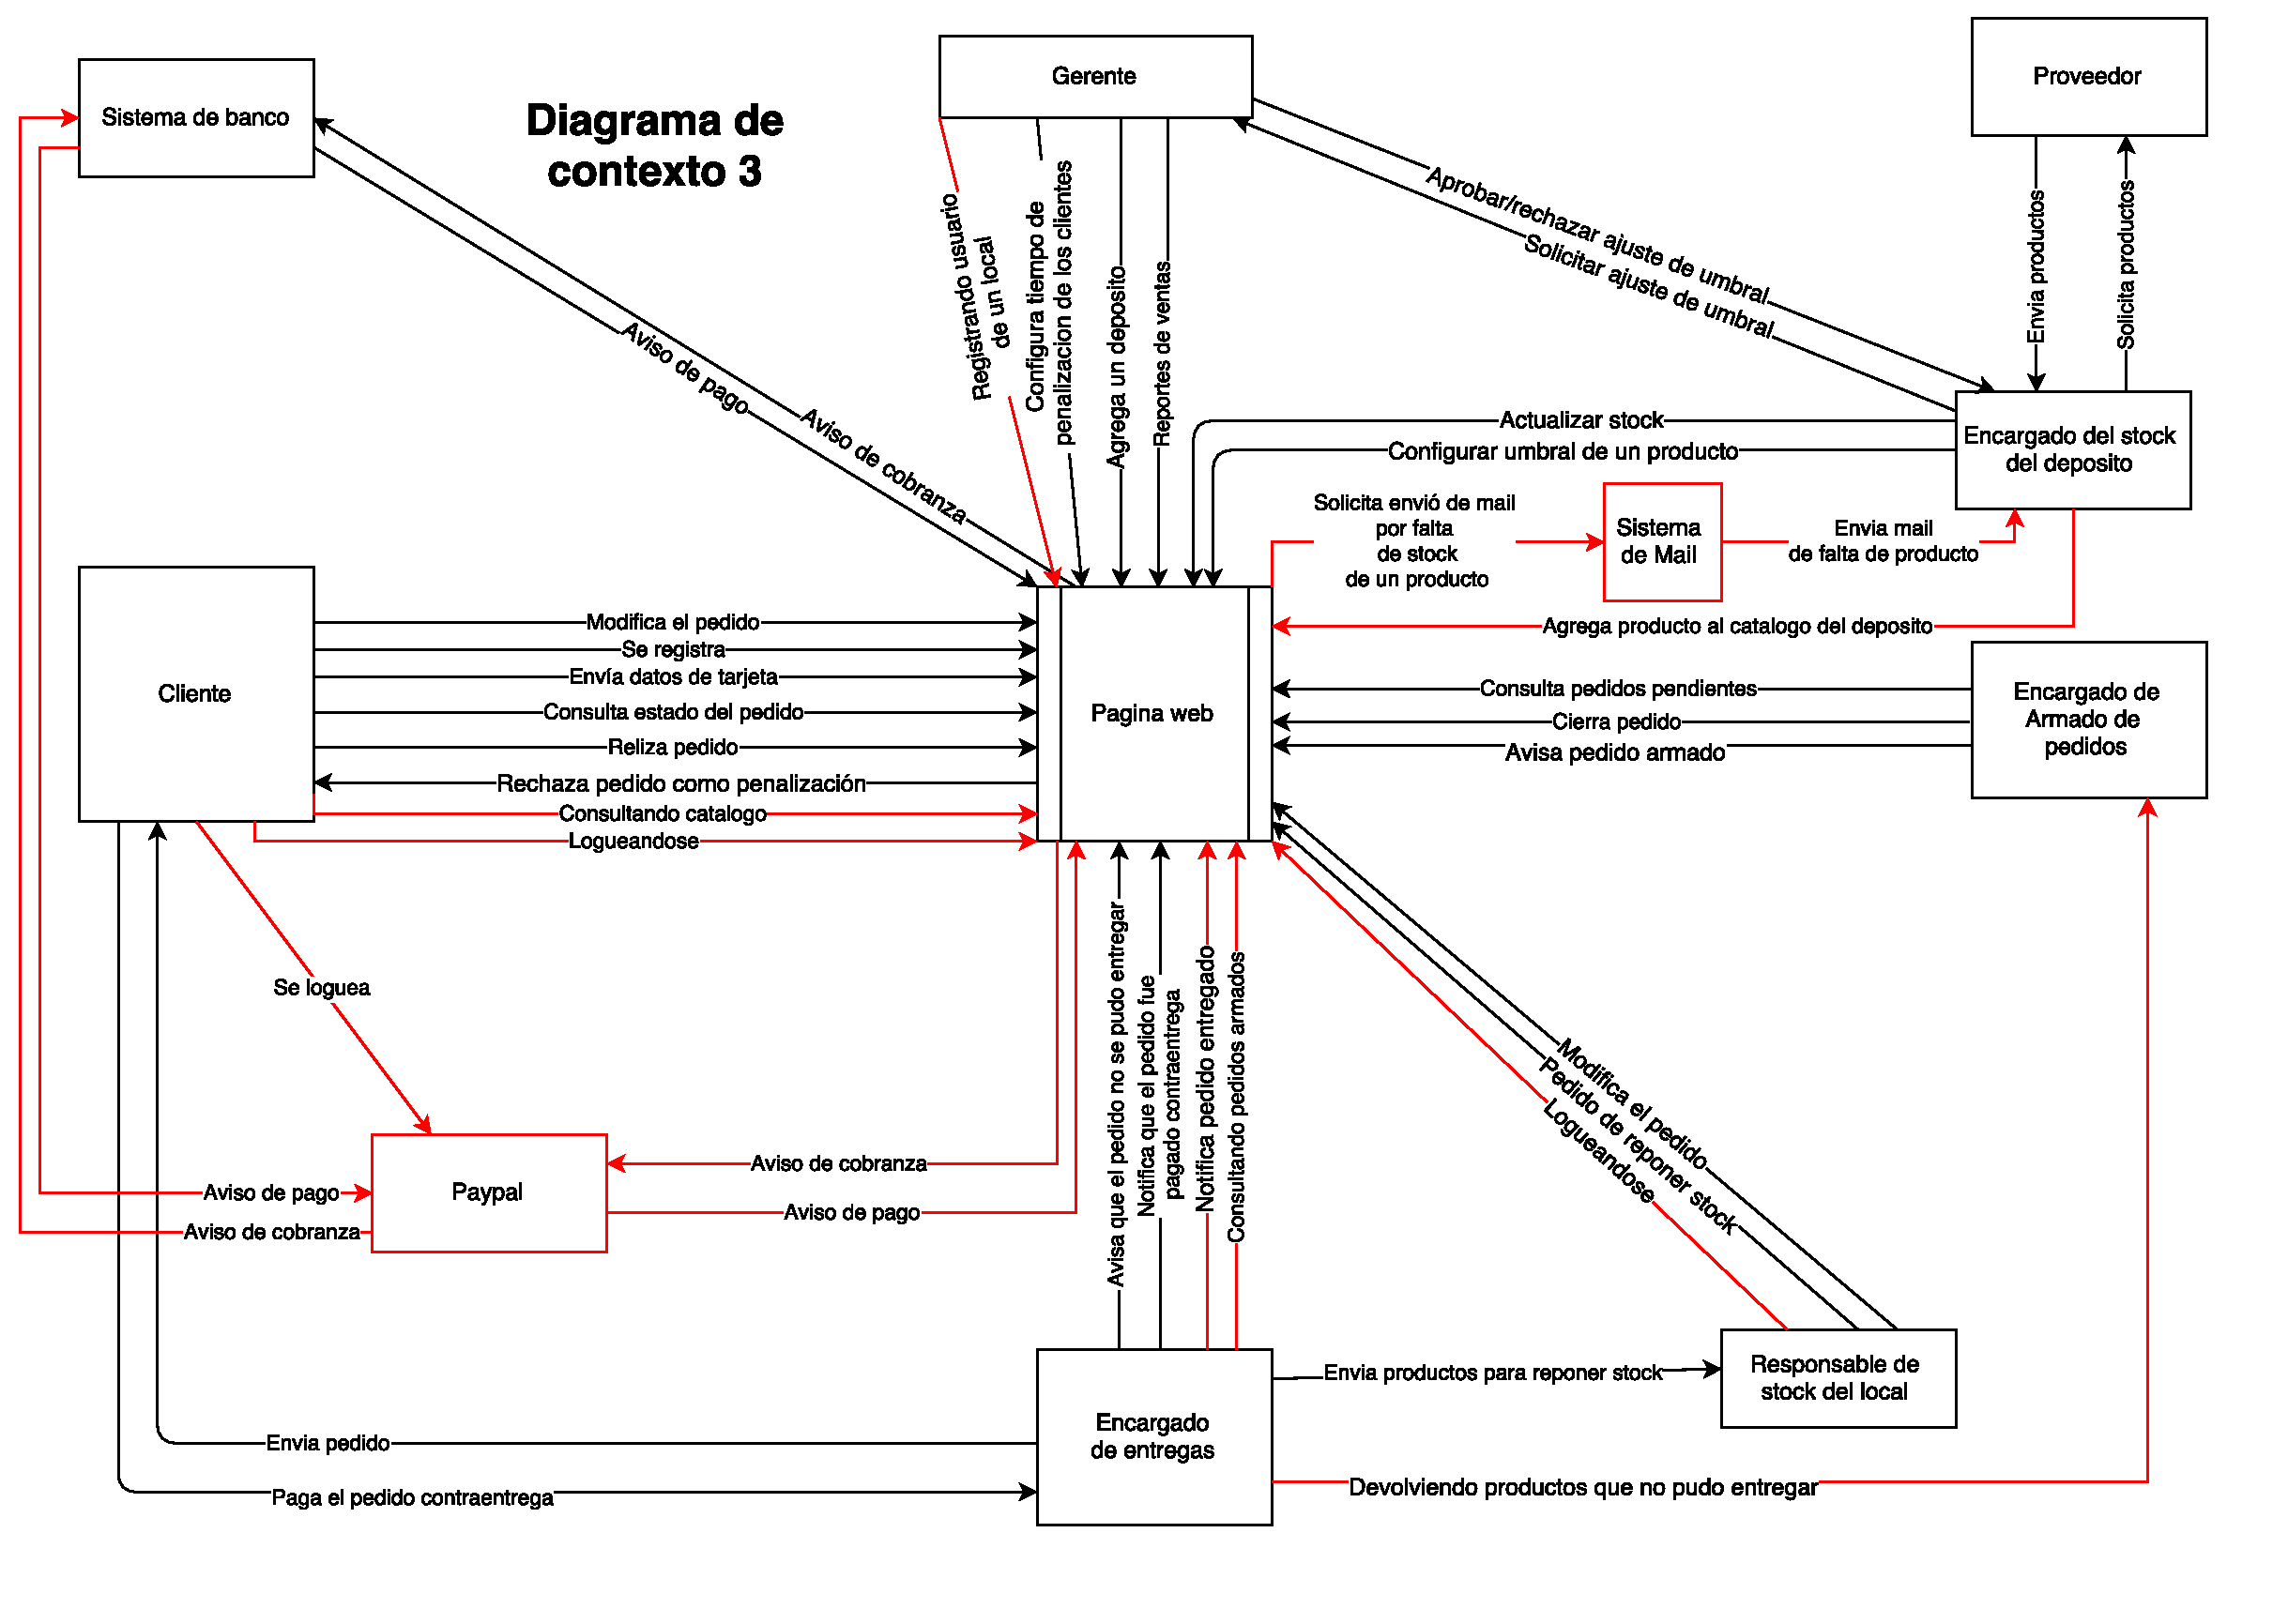
\includegraphics[scale=0.5, angle=90]{secciones/diagramaContexto}
% Acá debería figurar todo lo necesario como para que un lector no iniciado en el tema entienda el propósito general del sistema que van a describir. Puede citar algunos fragmentos del enunciado si lo consideran necesario, pero NO DEBE SER una copia del enunciado.

\section{Presunciones}

Primero listaremos las presunciones de dominio que realizamos en la primer instancia del trabajo:
\begin{enumerate}
\item El proveedor tiene stock infinito.
\item Los envíos a los locales siempre se realizan en horarios en los que hay empleados para recibirlos.
\item La información relevante que los dueños del sistema quieren se basa en estadísticas obtenidas a partir de las ventas online.
\item Los clientes, al registrarse, proporcionan un nombre de usuario, una contraseña, información de contacto y una foto con su DNI para confirmar su identidad.
\item Los locales también pueden modificar los pedidos que realizan en la página.
\item Todos los locales cuentan con dep\'ositos propios
\end{enumerate}

Estas presunciones nos resultaron suficientes, de modo que no hemos realizado ninguna presunción extra en esta nueva instancia del trabajo.

\newpage
% Acá deberían listar aquellas cuestiones que asumieron por encima del enunciado. Estas cuestiones pueden provenir de alguna consulta con docentes. También pueden provenir de alguna especulación o interpretación que el grupo hizo.


\section{Vistas}

\subsection{Modelo de operaciones}

\subsubsection{Diagrama de casos de uso}

En este primer modelo mostraremos todos los escenarios en los que algún agente (encargados, clientes, locales, gerente, etc) participa en alguna operación del sistema. A estos agentes los llamaremos actores y los representamos con la figura de una persona. También mostraremos las relaciones de extensión e inclusión entre las operaciones, en caso de que existan. Luego, detallaremos por completo los pasos que conlleva realizar cada una de las operaciones, es decir, como el actor (o actores) que participan en dicha operación interactúan con nuestro sistema. También se visualizan relaciones de herencia entre actores, donde los casos de uso del actor padre también pertenecen al actor hijo.

Si bien esta técnica detalla los pasos de una operación y muestra los actores que participan en cada una, no permite visualizar un orden a seguir entre operaciones ni tampoco modelar aspectos puros del sistema (comportamiento automático en donde no hay actores). El orden entre operaciones lo mostraremos más adelante, cuando utilicemos diagramas de actividad.

A continuación mostraremos el diagrama de casos de uso resultante y el detalle de las operaciones de cada uno de los casos:

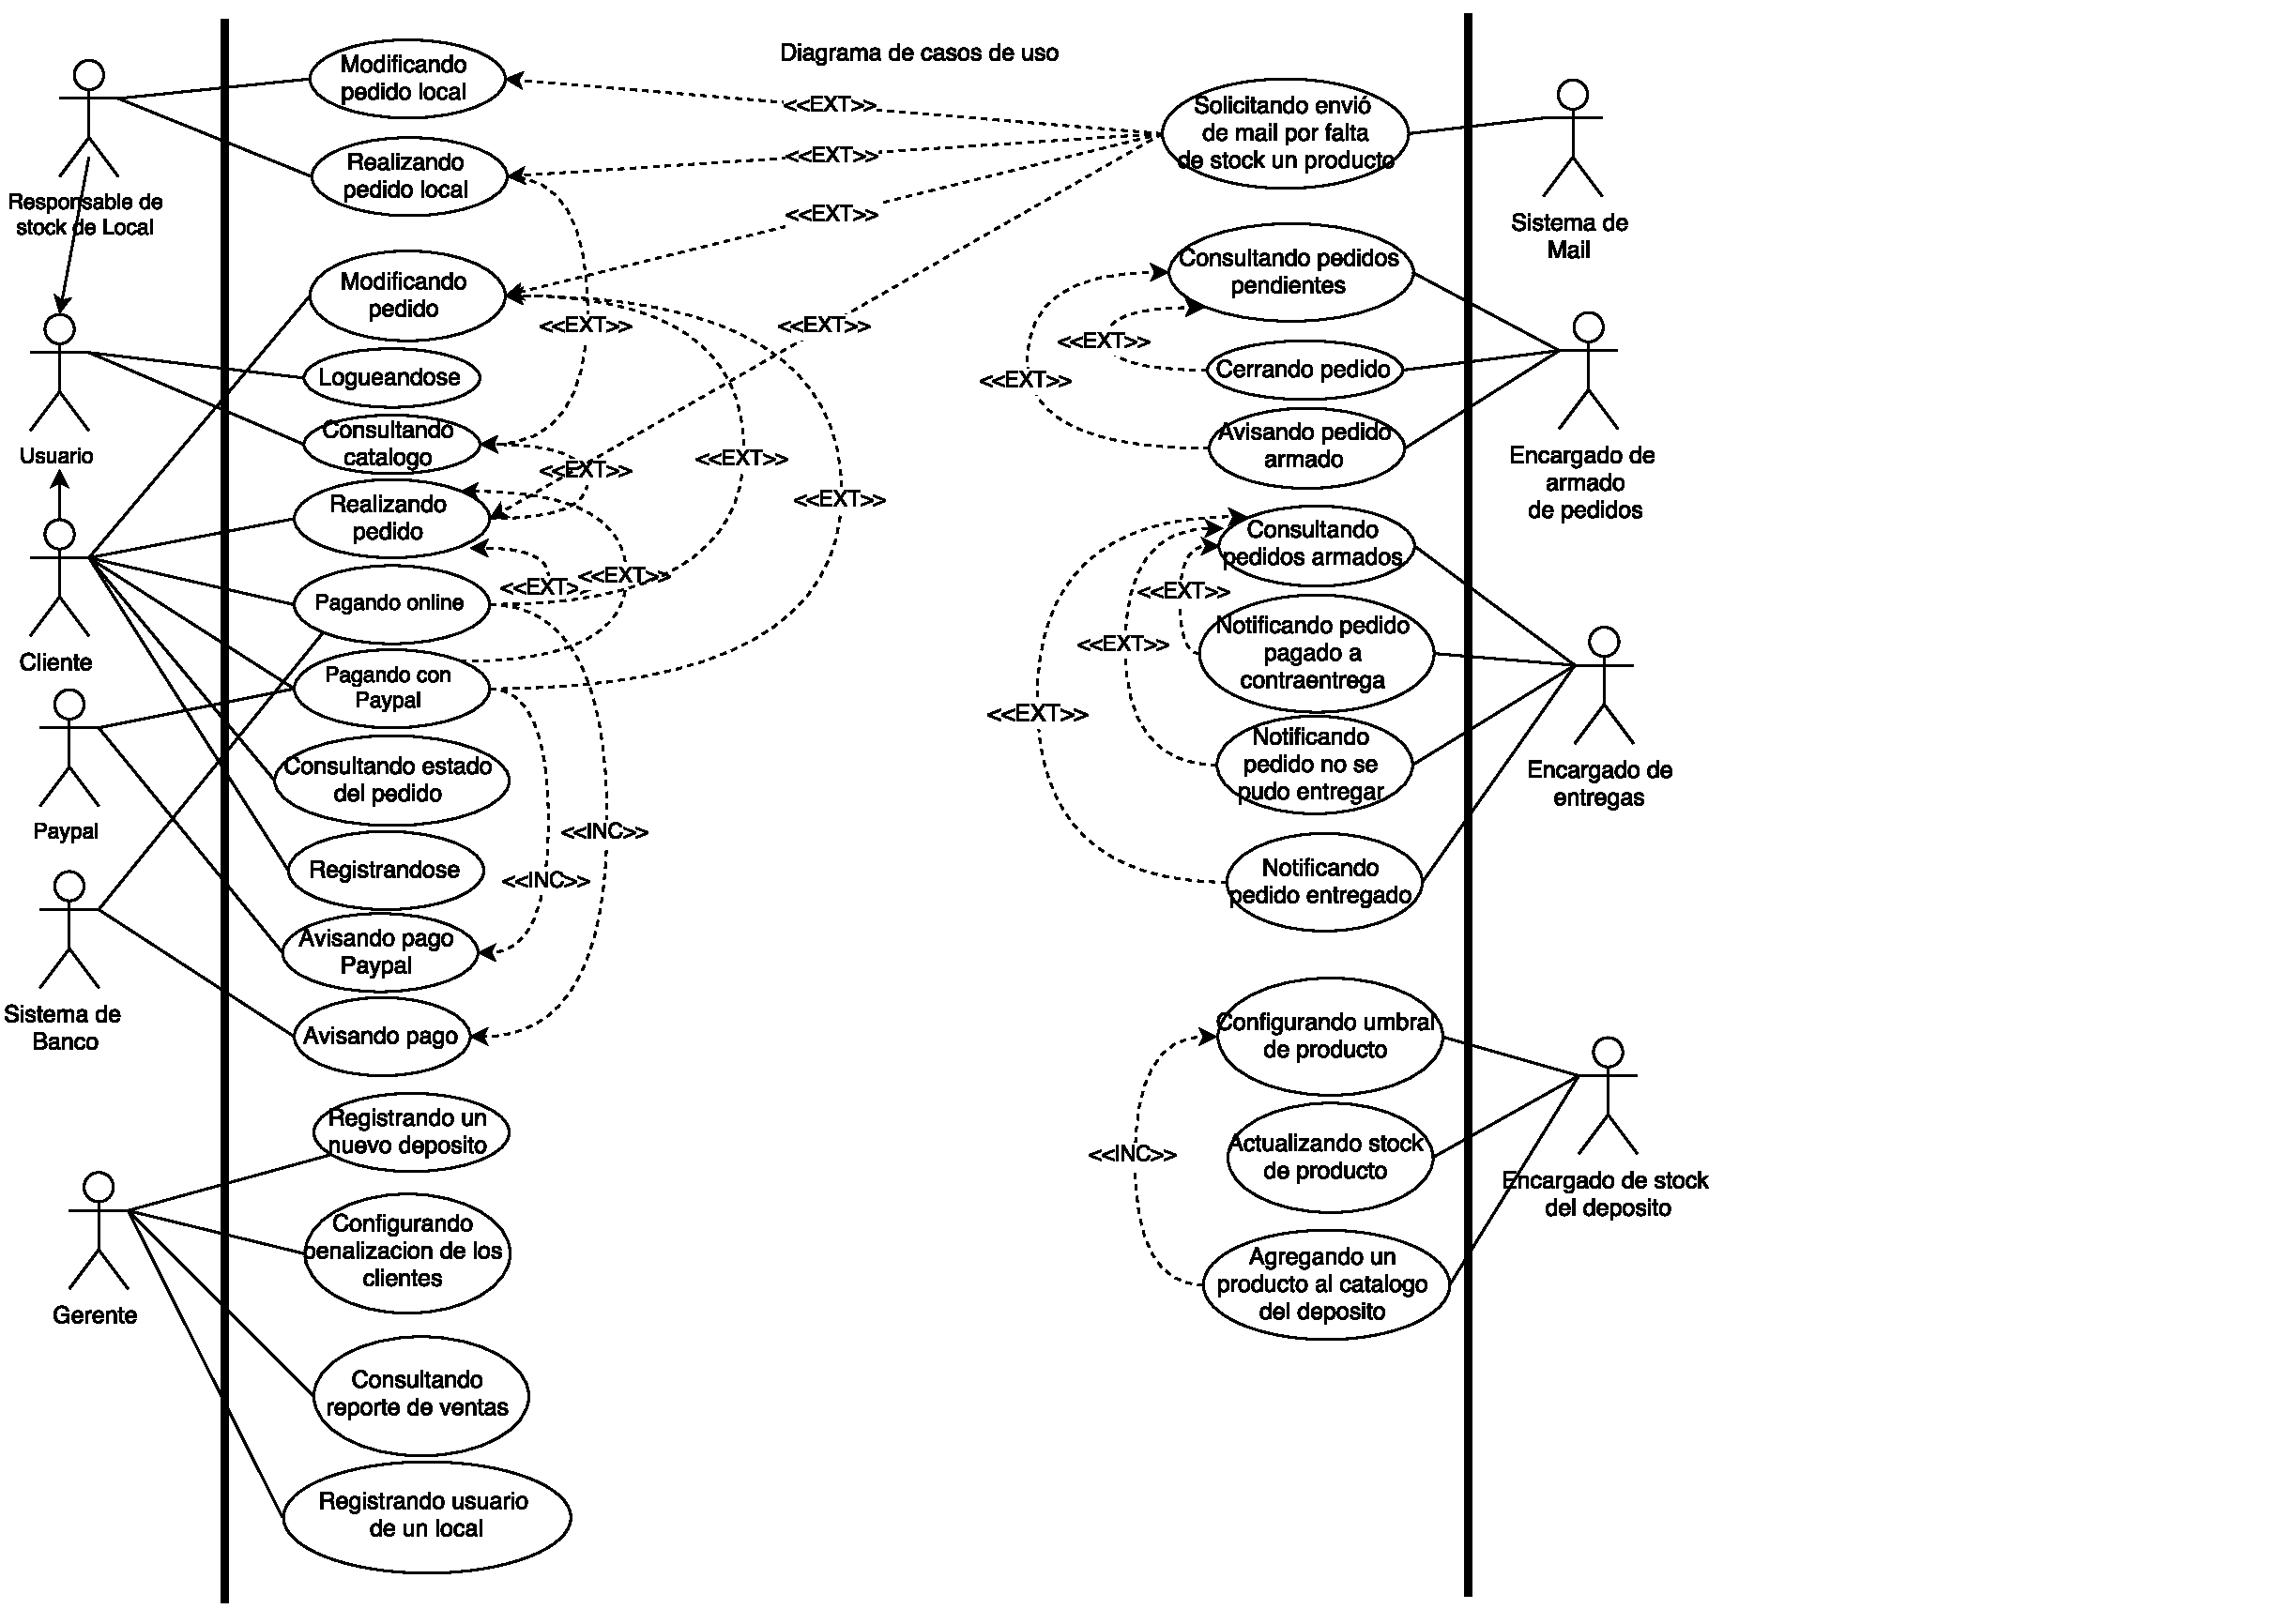
\includegraphics[scale=0.5, angle=90]{secciones/diagramaCasosUso}

\subsubsection{Detalle de los casos de uso}

\begin{tabular}{p{0.2\textwidth} p{0.8\textwidth}}
    \textsc{Caso de uso} & Registrándose \\
    \textsc{Actores} & Cliente \\
    \textsc{Pre} & - \\
    \textsc{Post} & El cliente se registra en el sitio \\
\end{tabular}

\begin{center}
\begin{tabular}{|p{0.4\textwidth}|p{0.4\textwidth}|}
    \hline
    \multicolumn{1}{|c|}{Curso Normal} &
    \multicolumn{1}{|c|}{Curso alternativo} \\
    \hline
    1. El cliente ingresa sus datos personales (nombre, apellido, DNI, domicilio y numero teléfono). & \\
    2. El cliente ingresa un nombre de usuario. & \\
    3. El cliente ingresa una contraseña. & \\
    4. El cliente sube al sitio una copia de su DNI. & \\
    5. El sistema valida que los datos ingresados no pertenezcan a un usuario
    existente. &
    5.1 Si los datos ya existen, volver al paso 1.  \\
    6. El sistema guarda los datos del usuario. & \\
    7. FIN CU. & \\
    \hline
\end{tabular}
\end{center}

\begin{tabular}{p{0.2\textwidth} p{0.8\textwidth}}
    \textsc{Caso de uso} & Logueandose \\
    \textsc{Actores} & Usuario \\
    \textsc{Pre} & El usuario debe estar registrado. \\
    \textsc{Post} & El usuario ingresa al sitio con su cuenta. \\
\end{tabular}

\begin{center}
\begin{tabular}{|p{0.4\textwidth}|p{0.4\textwidth}|}
    \hline
    \multicolumn{1}{|c|}{Curso Normal} &
    \multicolumn{1}{|c|}{Curso alternativo} \\
    \hline
    1. El usuario ingresa el nombre de su cuenta y su contraseña. & \\
    2. El sistema valida los datos. &
    2.1. Si los datos son incorrectos, volver al paso 1. \\
    3. FIN CU. & \\
    \hline
\end{tabular}
\end{center}

\begin{tabular}{p{0.2\textwidth} p{0.8\textwidth}}
    \textsc{Caso de uso} & Consultando catálogo. \\
    \textsc{Actores} & Usuario \\
    \textsc{Pre} & El usuario está logueado. \\
    \textsc{Post} & El usuario visualiza el catálogo de todos los productos
    disponibles. \\
\end{tabular}

\begin{center}
\begin{tabular}{|p{0.4\textwidth}|p{0.4\textwidth}|}
    \hline
    \multicolumn{1}{|c|}{Curso Normal} &
    \multicolumn{1}{|c|}{Curso alternativo} \\
    \hline
    1. El sistema muestra al usuario todos los productos disponibles en alguno de los depósitos del sistema y el stock disponible de cada uno en dicho depósito. & \\
    2. Si el usuario quiere realizar un pedido de productos. EXT CU:
    ``Realizando Pedido''. & \\
    3. FIN CU. & \\
    \hline
\end{tabular}
\end{center}

\begin{tabular}{p{0.2\textwidth} p{0.8\textwidth}}
    \textsc{Caso de uso} & Realizando pedido local. \\
    \textsc{Actores} & Responsable de stock del local \\
    \textsc{Pre} & El responsable de stock del local debe estar logueado y debe
    haber consultado el catálogo de productos previamente. \\
    \textsc{Post} & El responsable de stock del local realizó un pedido con
    éxito. \\
\end{tabular}

\begin{center}
\begin{tabular}{|p{0.4\textwidth}|p{0.4\textwidth}|}
    \hline
    \multicolumn{1}{|c|}{Curso Normal} &
    \multicolumn{1}{|c|}{Curso alternativo} \\
    \hline
    1. El sistema verifica que el responsable de stock del local no tenga un pedido pendiente de entrega. &
    1.1. Si el responsable de stock del local tiene un pedido pendiente, rechazar pedido. FIN CU. \\
    2. El responsable de stock del local selecciona el producto que desea
    adquirir. & \\
    3. El responsable de stock ingresa la cantidad de unidades que desea del
    producto. & \\
    4. El responsable de stock vuelve al paso 2 por cada producto que desea
    adquirir. & \\
    5. El responsable de stock confirma el pedido. & \\
    6. El sistema chequea que en el depósito haya suficiente stock disponible para cada producto solicitado en el pedido. &
    6.1. Si el stock disponible no es suficiente para alguno de los productos, mostrar al usuario un mensaje de error diciendo ``Stock insuficiente''. FIN CU. \\
    7. El sistema propone al responsable de stock tres posibles fechas al azar, en días hábiles, dentro de los próximos siete días para que le sea entregado su pedido. & \\
    8. El responsable de stock selecciona la fecha que desea en que le entreguen el pedido. & \\
    9. El sistema almacena los datos del pedido. & \\
	10. El sistema reserva en el depósito, por cada producto pedido, la cantidad solicitada de dicho producto. & \\
	11. Si el pedido causo que el stock de un producto sea menor que el umbral configurado para dicho producto, EXT CU: ``Solicitando envió de mail por falta de stock un producto''. & \\
	12. El sistema vuelve al paso 11 por cada producto que haya caído debajo de su umbral por causa de los productos pedidos. & \\
    13. FIN CU. & \\
    \hline
\end{tabular}
\end{center}

Es importante notar que el sistema solo arregla una fecha de entrega con el encargado de stock del local y no un horario. Es el encargado de entregas quien se encarga de entregar los pedidos a los locales en el horario en que estos operan.

\newpage

\begin{tabular}{p{0.2\textwidth} p{0.8\textwidth}}
    \textsc{Caso de uso} & Realizando Pedido. \\
    \textsc{Actores} & Cliente \\
    \textsc{Pre} & El Cliente está logueado y consultó el catálogo de
    productos. \\
    \textsc{Post} & El cliente realizó un pedido con éxito. \\
\end{tabular}


\begin{center}
\begin{tabular}{|p{0.4\textwidth}|p{0.4\textwidth}|}
    \hline
    \multicolumn{1}{|c|}{Curso Normal} &
    \multicolumn{1}{|c|}{Curso alternativo} \\
    \hline
    1. El sistema verifica que el cliente no esté penalizado. &
    1.1 Si el Cliente está penalizado, rechazar pedido. FIN CU. \\
    2. El sistema verifica que el cliente no tenga un pedido pendiente de entrega. &
    2.2 Si el Cliente tiene un pedido pendiente, rechazar pedido. FIN CU. \\
    3. El Cliente selecciona el producto que desea adquirir. & \\
    4. El Cliente ingresa la cantidad de unidades que desea del producto, la cual debe estar entre $1$ y el stock disponible en el depósito en ese momento. & \\
    5. El Cliente vuelve al paso 3 por cada producto que desea adquirir. & \\
    6. El sitio calcula el importe total del pedido. & \\
    7. El Cliente confirma el pedido. & \\
    8. El sistema chequea que en el depósito haya suficiente stock disponible para cada producto solicitado en el pedido. &
    8.1. Si el stock disponible no es suficiente para alguno de los productos, mostrar al cliente un mensaje de error diciendo ``Stock insuficiente''. FIN CU. \\
    9. El sistema propone al cliente tres posibles fechas al azar, en días hábiles, dentro de los próximos siete días para que le sea entregado su pedido. & \\
    10. El Cliente selecciona la fecha que desea en que le entreguen el pedido. & \\
    11. El Cliente selecciona el método de pago que desea entre Paypal, pagar con tarjeta de crédito o débito, o pagar a contraentrega. & \\
    12. Si el Cliente desea pagar con tarjeta de crédito o débito. EXT CU:
    ``Pagando Online''. & \\
    13. Si el Cliente desea pagar con PayPal. EXT CU: ``Pagando con PayPal''. & \\
    14. El sistema almacena los datos del pedido. & \\
    15. El sistema reserva en el depósito, por cada producto pedido, la cantidad solicitada de dicho producto. & \\
\end{tabular}
\end{center}

\begin{center}
\begin{tabular}{|p{0.4\textwidth}|p{0.4\textwidth}|}
    16. Si el pedido causo que el stock de un producto sea menor que el umbral configurado para dicho producto, EXT CU: ``Solicitando envió de mail por falta de stock un producto''. & \\
	17. El sistema vuelve al paso 16 por cada producto que haya caído debajo de su umbral por causa de los productos pedidos. & \\
    18. FIN CU. & \\
    \hline
\end{tabular}
\end{center}


Es importante notar que la cantidad de unidades de un producto que el cliente puede pedir es igual a la cantidad de unidades disponibles en el deposito en el momento que el cliente \textbf{inicia} el pedido. Esta cantidad pudo haber disminuido \textit{(por un pedido de otro usuario)} e impedir que el cliente concrete su pedido. En este caso, el cliente deberá iniciar la operación nuevamente.


Se verifica si el cliente está penalizado comprobando que haya una instancia de ``\textit{Penalización}'' asociada a la cuenta cuyo intervalo de fechas contenga a la fecha actual.
Se puede ver en más detalle el flujo de penalización en el modelo de máquinas de estado.


También existe un diagrama de actividad que muestra el orden completo del flujo de la realización de un pedido \textit{(por parte de un cliente)}, desde que se consulta el catálogo hasta que el pedido es entregado.

\vspace{2cm}

\begin{tabular}{p{0.2\textwidth} p{0.8\textwidth}}
    \textsc{Caso de uso} & Pagando Online. \\
    \textsc{Actores} & Cliente, Sistema de Banco \\
    \textsc{Pre} & El cliente está logueado y debe estar realizando un pedido. \\
    \textsc{Post} & El cliente realiza el pago del pedido vía online. \\
\end{tabular}

\begin{center}
\begin{tabular}{|p{0.4\textwidth}|p{0.4\textwidth}|}
    \hline
    \multicolumn{1}{|c|}{Curso Normal} &
    \multicolumn{1}{|c|}{Curso alternativo} \\
    \hline
    1. El cliente completa los datos de la tarjeta (tipo, nombre del titular,
    número, código de seguridad, fecha de vencimiento) &
    1.1 El usuario dejó algún campo en blanco. Se vuelve al paso 1. \\
     3. El sistema de banco valida los datos de la tarjeta del cliente. &
   3.1. Si el sistema de banco informa que los datos de la tarjeta no son válidos, volver al paso 1. \\
   4. El sistema envía al sistema de banco los datos de la tarjeta del cliente y el monto a cobrarle. & \\
   4. INC CU: ``Avisando pago''. & \\
   5. FIN CU. & \\
    \hline
\end{tabular}
\end{center}

\newpage

\begin{tabular}{p{0.2\textwidth} p{0.8\textwidth}}
    \textsc{Caso de uso} & Avisando pago. \\
    \textsc{Actores} & Sistema de Banco \\
    \textsc{Pre} & El sistema envió al sistema de banco los datos de tarjeta de un cliente y un monto a cobrar. \\
    \textsc{Post} & El sistema de banco confirma que el pago del monto se realizo correctamente. \\
\end{tabular}

\begin{center}
\begin{tabular}{|p{0.4\textwidth}|p{0.4\textwidth}|}
    \hline
    \multicolumn{1}{|c|}{Curso Normal} &
    \multicolumn{1}{|c|}{Curso alternativo} \\
    \hline
    1. El sistema de banco chequea que el pago se pueda realizar correctamente.
    &
    1.1. Si el sistema de banco informa que no se puede, el sistema muestra un mensaje de error. FIN CU \\
    2. El sistema de banco envía al sistema la nota de pago del pedido. & \\
    3. El sistema almacena la nota de pago. & \\
    4. El sistema marca el pedido como pagado. & \\
    5. FIN CU. & \\
    \hline
\end{tabular}
\end{center}

\begin{tabular}{p{0.2\textwidth} p{0.8\textwidth}}
    \textsc{Caso de uso} & Pagando con PayPal \\
    \textsc{Actores} & Cliente, PayPal \\
    \textsc{Pre} & El cliente está logueado y debe haber realizado un pedido.
    \\
    \textsc{Post} & El cliente realiza el pago del pedido vía PayPal. \\
\end{tabular}

\begin{center}
\begin{tabular}{|p{0.4\textwidth}|p{0.4\textwidth}|}
    \hline
    \multicolumn{1}{|c|}{Curso Normal} &
    \multicolumn{1}{|c|}{Curso alternativo} \\
    \hline
    1. El cliente completa los datos de su cuenta de PayPal. & \\
    2. El sistema envía a PayPal los datos de usuario y el monto a pagar. & \\
    3. PayPal chequea si los datos son correctos. &
    3.1. Si los datos de usuario son incorrectos, volver al paso 1. \\
    4. INC CU: ``Avisando pago PayPal''. & \\
    5. FIN CU. & \\
    \hline
\end{tabular}
\end{center}


\begin{tabular}{p{0.2\textwidth} p{0.8\textwidth}}
    \textsc{Caso de uso} & Avisando pago PayPal \\
    \textsc{Actores} & Cliente, PayPal \\
    \textsc{Pre} & El sistema envío a Paypal los datos de usuario de un cliente y el monto a cobrar. \\
    \textsc{Post} & Paypal confirma que el pago del monto se realizo correctamente. \\
\end{tabular}

\begin{center}
\begin{tabular}{|p{0.4\textwidth}|p{0.4\textwidth}|}
    \hline
    \multicolumn{1}{|c|}{Curso Normal} &
    \multicolumn{1}{|c|}{Curso alternativo} \\
    \hline
    1. Paypal chequea que el pago se pueda realizar correctamente. &
    1.1. Si el Paypal informa que no se puede, el sistema muestra un mensaje de error. FIN CU \\
    2. Paypal envía al sistema la nota de pago del pedido. & \\
    3. El sistema almacena la nota de pago. & \\
    4. El sistema marca el pedido como pagado. & \\
    5. FIN CU. & \\
    \hline
\end{tabular}
\end{center}

\newpage

\begin{tabular}{p{0.2\textwidth} p{0.8\textwidth}}
    \textsc{Caso de uso} & Consultando estado del pedido. \\
    \textsc{Actores} & Usuario \\
    \textsc{Pre} & El usuario está logueado y debe haber realizado un pedido.
    \\
    \textsc{Post} & El usuario visualiza el estado actual del pedido realizado. \\
\end{tabular}

\begin{center}
\begin{tabular}{|p{0.4\textwidth}|p{0.4\textwidth}|}
    \hline
    \multicolumn{1}{|c|}{Curso Normal} &
    \multicolumn{1}{|c|}{Curso alternativo} \\
    \hline
    1. El sitio muestra al usuario si su pedido está pagado o no. & \\
	2. Si el cliente realizó un pedido y este aún no fue cerrado, muestra el estado ``Pendiente''. Si el pedido se encuentra cerrado, muestra el estado ``Cerrado''. Si el pedido ya fue armado, muestra el estado ``Armado''. Si el pedido fue entregado, muestra el estado ``Entregado''. Si el pedido no fue entregado, muestra el estado ``No entregado'' & \\
	3. FIN CU. & \\
    \hline
\end{tabular}
\end{center}

\begin{tabular}{p{0.2\textwidth} p{0.8\textwidth}}
    \textsc{Caso de uso} & Modificando pedido. \\
    \textsc{Actores} & Cliente \\
    \textsc{Pre} & El cliente está logueado, debe haber realizado un pedido y
    que su \textbf{único} pedido esté sin cerrar. \\
    \textsc{Post} & El cliente logra modificar el pedido sin cerrar.
    \\
\end{tabular}

\begin{center}
\begin{tabular}{|p{0.4\textwidth}|p{0.4\textwidth}|}
    \hline
    \multicolumn{1}{|c|}{Curso Normal} &
    \multicolumn{1}{|c|}{Curso alternativo} \\
    \hline
	1. El Cliente selecciona el producto que desea adquirir. & \\
	2. El Cliente ingresa la cantidad de unidades que desea del producto, la cual debe estar entre $1$ y el stock disponible en el depósito en ese momento. Si este producto ya estaba en el pedido, la cantidad solicitada se suma a la cantidad pedida previamente. & \\
	3. El Cliente vuelve al paso 1 por cada producto que desea adquirir. & \\
	4. El sitio calcula el importe de los nuevos productos agregados al pedido y de las unidades adicionales pedidas de productos que ya estaban en el pedido. & \\
	5. El Cliente confirma el pedido. & \\
	6. El sistema chequea que en el depósito haya suficiente stock disponible para cada nuevo producto solicitado en el pedido y para las unidades extra de productos previamente solicitados. &
	6.1. Si el stock disponible no es suficiente para alguno de los productos, mostrar al usuario un mensaje de error diciendo ``Stock insuficiente'', reiniciar la lista de productos solicitados al estado anterior del pedido y volver al paso 1. \\
	7. Si cuando el Cliente realizo el pedido original eligió pagar con tarjeta de crédito o débito. EXT CU: ``Pagando Online''. & \\
\end{tabular}
\end{center}

\begin{center}
\begin{tabular}{|p{0.4\textwidth}|p{0.4\textwidth}|}
	8. Si cuando el Cliente realizo el pedido original eligió pagar con PayPal. EXT CU: ``Pagando con PayPal''. & \\
	9. El sistema almacena los nuevos datos del pedido. & \\
	10. El sistema reserva en el depósito, por cada producto pedido, la cantidad solicitada de dicho producto (si es un nuevo producto en el pedido) o la diferencia entre la cantidad anterior y la nueva cantidad solicitada (si es un producto que ya estaba en el pedido original). & \\
	11. Si el pedido causo que el stock de un producto sea menor que el umbral configurado para dicho producto, EXT CU: ``Solicitando envió de mail por falta de stock un producto''. & \\
	12. El sistema vuelve al paso 11 por cada producto que haya caído debajo de su umbral por causa de los nuevos productos pedidos. & \\
	13. FIN CU. & \\
    \hline
\end{tabular}
\end{center}
Es importante notar que solo permitimos que los clientes agreguen nuevos productos y/o que aumenten las unidades de los productos que ya pidieron, pero \textbf{no} permitimos que quiten cosas de su pedido original. Esto es debido a que estos productos ya pudieron haber sido pagados por el cliente \textit{(si es que eligió pagar online con tarjeta o con Paypal)}, y hemos decidido no hacer reembolsos.


\newpage

\begin{tabular}{p{0.2\textwidth} p{0.8\textwidth}}
    \textsc{Caso de uso} & Modificando pedido local. \\
    \textsc{Actores} & Responsable de stock del local. \\
    \textsc{Pre} & El responsable de stock del local debe haber realizado un pedido y
    que su \textbf{único} pedido esté sin cerrar. \\
    \textsc{Post} & El responsable de stock del local logra modificar el pedido sin cerrar.
    \\
\end{tabular}

\begin{center}
\begin{tabular}{|p{0.4\textwidth}|p{0.4\textwidth}|}
    \hline
    \multicolumn{1}{|c|}{Curso Normal} &
    \multicolumn{1}{|c|}{Curso alternativo} \\
    \hline
	1. El responsable de stock del local selecciona el producto que desea adquirir. & \\
	2. El responsable de stock del local ingresa la cantidad de unidades que desea del producto, la cual debe estar entre $1$ y el stock disponible en el depósito en ese momento. Si este producto ya estaba en el pedido, la cantidad solicitada se suma a la cantidad pedida previamente. & \\
	3. El responsable de stock del local vuelve al paso 1 por cada producto que desea adquirir. & \\
	4. El responsable de stock del local confirma el pedido. & \\
	5. El sistema chequea que en el depósito haya suficiente stock disponible para cada nuevo producto solicitado en el pedido y para las unidades extra de productos previamente solicitados. &
	5.1. Si el stock disponible no es suficiente para alguno de los productos, mostrar al usuario un mensaje de error diciendo ``Stock insuficiente'', reiniciar la lista de productos solicitados al estado anterior del pedido y volver al paso 1. \\
	6. El sistema almacena los nuevos datos del pedido. & \\
	7. El sistema reserva en el depósito, por cada producto pedido, la cantidad solicitada de dicho producto (si es un nuevo producto en el pedido) o la diferencia entre la cantidad anterior y la nueva cantidad solicitada (si es un producto que ya estaba en el pedido original). & \\
	8. Si el pedido causo que el stock de un producto sea menor que el umbral configurado para dicho producto, EXT CU: ``Solicitando envió de mail por falta de stock un producto''. & \\
	9. El sistema vuelve al paso 8 por cada producto que haya caído debajo de su umbral por causa de los nuevos productos pedidos. & \\
	10. FIN CU. & \\
    \hline
\end{tabular}
\end{center}

A los locales tampoco les permitimos quitar productos de sus pedidos. El porque de esta decisión se explica en detalle en la sección \textbf{Discusión}.


\begin{tabular}{p{0.2\textwidth} p{0.8\textwidth}}
    \textsc{Caso de uso} & Registrando un nuevo depósito. \\
    \textsc{Actores} & Gerente \\
    \textsc{Pre} & - \\
    \textsc{Post} & El gerente agrega un nuevo depósito correctamente al sistema. \\
\end{tabular}

\begin{center}
\begin{tabular}{|p{0.4\textwidth}|p{0.4\textwidth}|}
    \hline
    \multicolumn{1}{|c|}{Curso Normal} &
    \multicolumn{1}{|c|}{Curso alternativo} \\
    \hline
    1. El gerente ingresa domicilio y teléfono del nuevo depósito. & \\
    2. El sistema valida que el domicilio y el teléfono ingresados no estén asignados a otro deposito y que sean validos. &
    2.1. Si los datos ingresados ya están en uso o no son validos, volver al paso 1. \\
    3. El sistema guarda la información del nuevo deposito. & \\
    4. FIN CU. & \\
    \hline
\end{tabular}
\end{center}


\vspace{2cm}

\begin{tabular}{p{0.2\textwidth} p{0.8\textwidth}}
    \textsc{Caso de uso} & Configurando penalización de los clientes. \\
    \textsc{Actores} & Gerente \\
    \textsc{Pre} & - \\
    \textsc{Post} & El gerente configura el sistema de penalización para los
    clientes. \\
\end{tabular}

\begin{center}
\begin{tabular}{|p{0.4\textwidth}|p{0.4\textwidth}|}
    \hline
    \multicolumn{1}{|c|}{Curso Normal} &
    \multicolumn{1}{|c|}{Curso alternativo} \\
    \hline
    1. El gerente ingresa el tiempo que dura la penalización de los clientes. &
    \\
    2. El sistema valida que el tiempo ingresado sea un numero entero mayor a uno. &
    2.1. Si el valor ingresado no es valido, volver al paso 1. \\
    3. El sistema guarda los datos ingresados. & \\
    4. FIN CU. & \\
    \hline
\end{tabular}
\end{center}

\newpage

\begin{tabular}{p{0.2\textwidth} p{0.8\textwidth}}
    \textsc{Caso de uso} & Consultando reporte de ventas. \\
    \textsc{Actores} & Gerente \\
    \textsc{Pre} & - \\
    \textsc{Post} & El gerente visualiza los reportes de ventas. \\
\end{tabular}

\begin{center}
\begin{tabular}{|p{0.4\textwidth}|p{0.4\textwidth}|}
    \hline
    \multicolumn{1}{|c|}{Curso Normal} &
    \multicolumn{1}{|c|}{Curso alternativo} \\
    \hline
    1. El gerente selecciona el tipo de reporte que desea ver. & \\
    2. Si selecciono el tipo ``Productos mas vendidos'', el sistema deberá generar y mostrar un listado de todos los productos del catalogo ordenados en forma decreciente según cuantas unidades de cada producto fueron pedidas en base a todos los pedidos realizados al sistema. & \\
    3. Si selecciono el tipo ``Depósitos con mas pedidos'' el sistema deberá generar y mostrar un listado de todos los depósitos registrados en el sistema ordenado en forma decreciente según cuantos pedidos se haya realizado en cada uno de ellos. & \\
    4. Si selecciono el tipo ``Métodos de pago'' el sistema deberá generar y mostrar una tabla indicando, para cada uno de los métodos de pago ofrecidos (Tarjeta online, Paypal o contraentrega), cuantos pedidos utilizaron dicho método de pago. & \\
    5. Si el gerente desea ver otro reporte de ventas, volver al paso 1. & \\
    6. FIN CU. & \\
    \hline
\end{tabular}
\end{center}

\vspace{2cm}

\begin{tabular}{p{0.2\textwidth} p{0.8\textwidth}}
    \textsc{Caso de uso} & Registrando usuario de un local. \\
    \textsc{Actores} & Gerente \\
    \textsc{Pre} & - \\
    \textsc{Post} & El gerente logra registrar un local correctamente. \\
\end{tabular}

\begin{center}
\begin{tabular}{|p{0.4\textwidth}|p{0.4\textwidth}|}
    \hline
    \multicolumn{1}{|c|}{Curso Normal} &
    \multicolumn{1}{|c|}{Curso alternativo} \\
    \hline
    1. El gerente ingresa un nombre de usuario &\\
    2. El gerente ingresa una contraseña. & \\
    3. El gerente ingresa los datos de local (dirección y teléfono). & \\
    4. El sistema valida los datos ingresados. & 
    4.1. Si el nombre de usuario ingresado ya esta en uso, volver al paso 1.\\
    5. El sistema guarda los datos ingresados. & \\
    6. FIN CU. & \\
    \hline
\end{tabular}
\end{center}

\begin{tabular}{p{0.2\textwidth} p{0.8\textwidth}}
    \textsc{Caso de uso} & Consultando pedidos pendientes. \\
    \textsc{Actores} & Encargado de armado de pedidos \\
    \textsc{Pre} & - \\
    \textsc{Post} & El encargado de armar pedidos logra visualizar los pedidos
    pendientes. \\
\end{tabular}

\begin{center}
\begin{tabular}{|p{0.4\textwidth}|p{0.4\textwidth}|}
    \hline
    \multicolumn{1}{|c|}{Curso Normal} &
    \multicolumn{1}{|c|}{Curso alternativo} \\
    \hline
    1. El sistema lista los pedidos pendientes al Encargado de armado de
    pedidos. & \\
    2. Si el Encargado de armado de pedidos quiere cerrar un pedido. EXT CU:
    ``Cerrando pedido''. & \\
    3. Si el Encargado de armado de pedidos quiere notificar que un pedido ya
    fue armado. EXT CU: ``Avisando pedido armado''. & \\
    4. FIN CU. & \\
    \hline
\end{tabular}
\end{center}

\begin{tabular}{p{0.2\textwidth} p{0.8\textwidth}}
    \textsc{Caso de uso} & Cerrando pedido. \\
    \textsc{Actores} & Encargado de armado de pedidos \\
    \textsc{Pre} & El Encargado de armado de pedidos seleccionó un pedido
    pendiente. \\
    \textsc{Post} & Se marca un pedido como cerrado. \\
\end{tabular}

\begin{center}
\begin{tabular}{|p{0.4\textwidth}|p{0.4\textwidth}|}
    \hline
    \multicolumn{1}{|c|}{Curso Normal} &
    \multicolumn{1}{|c|}{Curso alternativo} \\
    \hline
    1. El encargado de armado de pedidos marca al pedido como cerrado. & \\
    2. El sistema guarda el nuevo estado del pedido. & \\
    3. FIN CU. & \\
    \hline
\end{tabular}
\end{center}


\begin{tabular}{p{0.2\textwidth} p{0.8\textwidth}}
    \textsc{Caso de uso} & Avisando pedido armado. \\
    \textsc{Actores} & Encargado de armado de pedidos \\
    \textsc{Pre} & El Encargado de armado de pedidos seleccionó un pedido
    pendiente. \\
    \textsc{Post} & Se marca un pedido como armado. \\
\end{tabular}

\begin{center}
\begin{tabular}{|p{0.4\textwidth}|p{0.4\textwidth}|}
    \hline
    \multicolumn{1}{|c|}{Curso Normal} &
    \multicolumn{1}{|c|}{Curso alternativo} \\
    \hline
    1. El encargado de armado de pedidos marca al pedido como armado. & \\
    2. El sistema guarda el estado del pedido. & \\
    3. FIN CU. & \\
    \hline
\end{tabular}
\end{center}

\newpage

\begin{tabular}{p{0.2\textwidth} p{0.8\textwidth}}
    \textsc{Caso de uso} & Consultando pedidos armados. \\
    \textsc{Actores} & Encargado de entregas \\
    \textsc{Pre} & - \\
    \textsc{Post} & Se listan los pedidos que fueron armados. \\
\end{tabular}

\begin{center}
\begin{tabular}{|p{0.4\textwidth}|p{0.4\textwidth}|}
    \hline
    \multicolumn{1}{|c|}{Curso Normal} &
    \multicolumn{1}{|c|}{Curso alternativo} \\
    \hline
    1. El sistema muestra al Encargado de entregas el listado de pedidos
    armados. & \\
    2. Si el Encargado de entregas quiere notificar que un pedido fue pagado a
    contraentrega EXT CU ``Notificando pedido pagado a contraentrega''. & \\
    3. Si el Encargado de entregas quiere notificar que un pedido fue
    entregado EXT CU ``Notificando pedido entregado''. & \\
    4. Si el Encargado de entregas quiere notificar que un pedido no se pudo
    entregar EXT CU ``Notificando pedido no se pudo entregar''. & \\
    5. FIN CU. & \\
    \hline
\end{tabular}
\end{center}

\begin{tabular}{p{0.2\textwidth} p{0.8\textwidth}}
    \textsc{Caso de uso} & Notificando pedido entregado. \\
    \textsc{Actores} & Encargado de entregas \\
    \textsc{Pre} & Se seleccionó un pedido armado. \\
    \textsc{Post} & Se notifica en el sistema que el pedido se entregó. \\
\end{tabular}

\begin{center}
\begin{tabular}{|p{0.4\textwidth}|p{0.4\textwidth}|}
    \hline
    \multicolumn{1}{|c|}{Curso Normal} &
    \multicolumn{1}{|c|}{Curso alternativo} \\
    \hline
    1. El encargado de entregas marca el pedido como entregado. & \\
    2. El sistema guarda el nuevo estado del pedido y la fecha actual. & \\
    3. FIN CU. & \\
    \hline
\end{tabular}
\end{center}

\begin{tabular}{p{0.2\textwidth} p{0.8\textwidth}}
    \textsc{Caso de uso} & Notificando pedido pagado a contraentrega. \\
    \textsc{Actores} & Encargado de entregas \\
    \textsc{Pre} & Se seleccionó un pedido armado. \\
    \textsc{Post} & Se notifica en el sistema que el pedido se pagó a
    contraentrega. \\
\end{tabular}

\begin{center}
\begin{tabular}{|p{0.4\textwidth}|p{0.4\textwidth}|}
    \hline
    \multicolumn{1}{|c|}{Curso Normal} &
    \multicolumn{1}{|c|}{Curso alternativo} \\
    \hline
    1. El Encargado de entregas marca el pedido como pagado a contraentrega. & \\
    2. El sistema guarda el nuevo estado del pedido y la fecha actual. & \\
    3. FIN CU. & \\
    \hline
\end{tabular}
\end{center}

\newpage

\begin{tabular}{p{0.2\textwidth} p{0.8\textwidth}}
    \textsc{Caso de uso} & Notificando pedido no se pudo entregar. \\
    \textsc{Actores} & Encargado de entregas \\
    \textsc{Pre} & Se seleccionó un pedido armado. \\
    \textsc{Post} & Se notifica en el sistema que el pedido no se pudo
    entregar. \\
\end{tabular}

\begin{center}
\begin{tabular}{|p{0.4\textwidth}|p{0.4\textwidth}|}
    \hline
    \multicolumn{1}{|c|}{Curso Normal} &
    \multicolumn{1}{|c|}{Curso alternativo} \\
    \hline
    1. El Encargado de entregas marca un pedido como no entregado. & \\
    2. El Encargado de entregas ingresa el motivo de no haber podido entregar el pedido. & \\
    3. El sistema guarda el motivo, el nuevo estado del pedido y la fecha actual. & \\
    4. FIN CU. & \\
    \hline
\end{tabular}
\end{center}

\begin{tabular}{p{0.2\textwidth} p{0.8\textwidth}}
    \textsc{Caso de uso} & Configurando umbral de producto. \\
    \textsc{Actores} & Encargado de stock del depósito \\
    \textsc{Pre} & - \\
    \textsc{Post} & Se configura umbral para el depósito. \\
\end{tabular}

\begin{center}
\begin{tabular}{|p{0.4\textwidth}|p{0.4\textwidth}|}
    \hline
    \multicolumn{1}{|c|}{Curso Normal} &
    \multicolumn{1}{|c|}{Curso alternativo} \\
    \hline
    1. El Encargado de stock del depósito ingresa un código de producto. &
    1.1 Si el código es inválido volver a paso 1. \\
    2. El Encargado de stock del depósito ingresa un umbral para el producto. &
    \\
    3. El sistema guarda los datos ingresados. & \\
    4. FIN CU. & \\
    \hline
\end{tabular}
\end{center}

\begin{tabular}{p{0.2\textwidth} p{0.8\textwidth}}
    \textsc{Caso de uso} & Actualizando stock de producto. \\
    \textsc{Actores} & Encargado de stock del depósito \\
    \textsc{Pre} & - \\
    \textsc{Post} & El stock es actualizado. \\
\end{tabular}

\begin{center}
\begin{tabular}{|p{0.4\textwidth}|p{0.4\textwidth}|}
    \hline
    \multicolumn{1}{|c|}{Curso Normal} &
    \multicolumn{1}{|c|}{Curso alternativo} \\
    \hline
    1. El Encargado de stock del depósito ingresa el código de un producto y el
    nuevo stock & 
    1.1. Si el código ingresado no corresponde a un producto en el catalogo del deposito, mostrar un mensaje de error. Fin CU. \\
    2. El sistema suma al stock previo del producto el valor ingresado. & \\
    3. FIN CU. & \\
    \hline
\end{tabular}
\end{center}

\newpage

\begin{tabular}{p{0.2\textwidth} p{0.8\textwidth}}
    \textsc{Caso de uso} & Agregando un producto al catalogo del depósito. \\
    \textsc{Actores} & Encargado de stock del depósito \\
    \textsc{Pre} & -\\
    \textsc{Post} & El stock del producto se actualiza al valor ingresado. \\
\end{tabular}

\begin{center}
\begin{tabular}{|p{0.4\textwidth}|p{0.4\textwidth}|}
    \hline
    \multicolumn{1}{|c|}{Curso Normal} &
    \multicolumn{1}{|c|}{Curso alternativo} \\
    \hline
    1. El Encargado de stock del depósito ingresa el código de un producto y el nuevo stock & \\
    2. El sistema almacena el nuevo stock, sobreescribiendo el valor si ya existía. &
    \\
    3. Incluye CU: Configurando Umbral de Producto & \\
    4. FIN CU. & \\
    \hline
\end{tabular}
\end{center}

\begin{tabular}{p{0.2\textwidth} p{0.8\textwidth}}
    \textsc{Caso de uso} & Solicitando envío de mail por falta de stock de un producto. \\
    \textsc{Actores} & Sistema de mail \\
    \textsc{Pre} & Se activo la alarma de falta de stock de un producto. \\
    \textsc{Post} & El sistema de mail envía un aviso al encargado de stock del deposito. \\
\end{tabular}

\begin{center}
\begin{tabular}{|p{0.4\textwidth}|p{0.4\textwidth}|}
    \hline
    \multicolumn{1}{|c|}{Curso Normal} &
    \multicolumn{1}{|c|}{Curso alternativo} \\
    \hline
    1. El sistema le indica al sistema de mail que envíe un mail al encargado de stock del depósito para informarlo de cual producto falta stock y cuantas unidades quedan. & \\
    2. El sistema de mail envía el mail solicitado. & \\
	3. FIN CU. & \\
    \hline
\end{tabular}
\end{center}


\subsubsection{Trazabilidad}

A continuación listamos los requerimientos que se modelan con este diagrama.

\begin{itemize}
\item \textbf{Agregar depósitos al sistema:} Modelado con el CU: Registrando nuevo deposito
\item \textbf{Los usuarios se pueden autentificar:} Modelado con el CU: Logueandose
\item \textbf{Que el cliente envíe una copia del DNI mediante el sitio:} Modelado con el CU: Registrándose
\item \textbf{Cerrar un pedido desde la pagina web:} Modelado con el CU: Cerrando Pedido
\item \textbf{Tomar productos del pedido => Notificar pedido armado:} Modelado con el CU: Avisando Pedido Armado
\item \textbf{Configurar umbrales por producto en el sistema:} Modelado con el CU: Configurando umbral del producto.
\item \textbf{Incrementar stock cuando recibo reposición del proveedor:} Modelado con el CU: Actualizando stock de producto
\item \textbf{Coordinar fecha de entrega:} Modelado con el CU: Realizando Pedidos.
\item \textbf{Se puede consultar los registros de las ventas:} Modelado con el CU: Consultando Reportes de ventas
\item \textbf{Se puede configurar los parámetros del reporte:} Modelado con el CU: Consultando Reportes de ventas
\item \textbf{Los locales puedan registrarse:} Modelado con el CU: Registrando usuario de un local
\item \textbf{Los locales pueden y ver y seleccionar los productos que desea recibir:} Modelado con el CU: Consultando catalogo y Realizando Pedido
\item \textbf{Los locales pueden modificar los pedidos no cerrados:} Modelado con el CU: Modificando Pedido
\item \textbf{Los clientes pueden y ver y seleccionar los productos que desean recibir:} Modelado con el CU: Consultando Catalogo

\item \textbf{Los clientes pueden modificar los pedido no cerrados:} Modelado con el CU: Modificando Pedido
\item \textbf{Un cliente pueda registrarse:} Modelado con el CU: Registrándose
\item \textbf{Un cliente pueda seleccionar la fecha de entrega:} Modelado con el CU:  Realizando pedido
\item \textbf{Un cliente pueda ingresar sus datos de contacto:} Modelado con el CU: Registrándose
\item \textbf{Reservar stock:} Modelado con el CU: Realizar Pedido
\item \textbf{Los productos en falta son filtrado del listado que ve el cliente:} Modelado con el CU: Consultar Catalogo
\item \textbf{La cantidad máxima permitida para pedir un producto es igual a la que hay en el deposito:} Modelado con el CU: Realizar Pedido
\item \textbf{Consultar pedidos armados:} Modelado con el CU: Consultar Pedidos Armados
\item \textbf{Seleccionar pedido entregado:} Modelado con el CU: Notificar Pedido Entregado
\item \textbf{El cliente pago en contra-entrega => se notifica pago a contra-entrega:} Modelado con el CU: Notifica pedido pagado a contra-entrega
\item \textbf{El cliente pago desde la pagina => se notifica el pago online:} Modelado con el CU: Avisando Pago
\item \textbf{Coordinar fecha de entrega con proveedor:} Modelado con el CU: Actualizar Stock de un producto
\item \textbf{Llevar el conteo en base a los pedidos realizados de cuantos productos quedan:} Modelado con el CU: Realizar Pedido
\item \textbf{Cliente pague el pedido:} Modelado con el CU: Pagando online y Pagando con PayPal
\item \textbf{Ofrecer pago con PayPal:} Modelado con el CU: Pagando con PayPal
\item \textbf{Ofrecer pago con crédito:} Modelado con el CU: Pagando online
\item \textbf{Ofrecer pago con débito:} Modelado con el CU: Pagando online
\item \textbf{Ofrecer pago con efectivo:} Modelado con el CU: Notificando pedido pagado a contra-entrega
 
\end{itemize}

\newpage

\subsection{Modelo conceptual}

\subsubsection{Diagrama de clases}

En este modelo se podrá visualizar los conceptos más importantes del sistema. A estos conceptos los llamaremos clases, las cuales tienen atributos que caracterizan a dicho concepto. También mostraremos las relaciones entre estas clases, el tipo de relación (uno a uno, uno a muchos, muchos a muchos, etc), el rol de cada clase en la relación, clases de asociación en la relación y los casos de herencia entre clases.
Luego, usaremos OCL para realizar restricciones de instanciación de las clases.

En este diagrama mostramos la información que almacena el sistema:
\begin{itemize}
\item Historial de pedidos realizados por un cliente.
\item Historial de pedidos realizados por un local.
\item Información de cada pedido: estado, fecha de entrega, método de pago, productos pedidos y su cantidad, depósito que atendió el pedido, etc.
\item Configuración de los umbrales de cada depósito (por producto).
\item Stock reservado y disponible de cada depósito (por producto).
\item Historial de penalización de cada usuario.
\item Datos personales de cada usuario.
\item Datos de cada depósito.
\end{itemize}

A continuación mostraremos el diagrama de clases y las restricciones OCL realizadas:

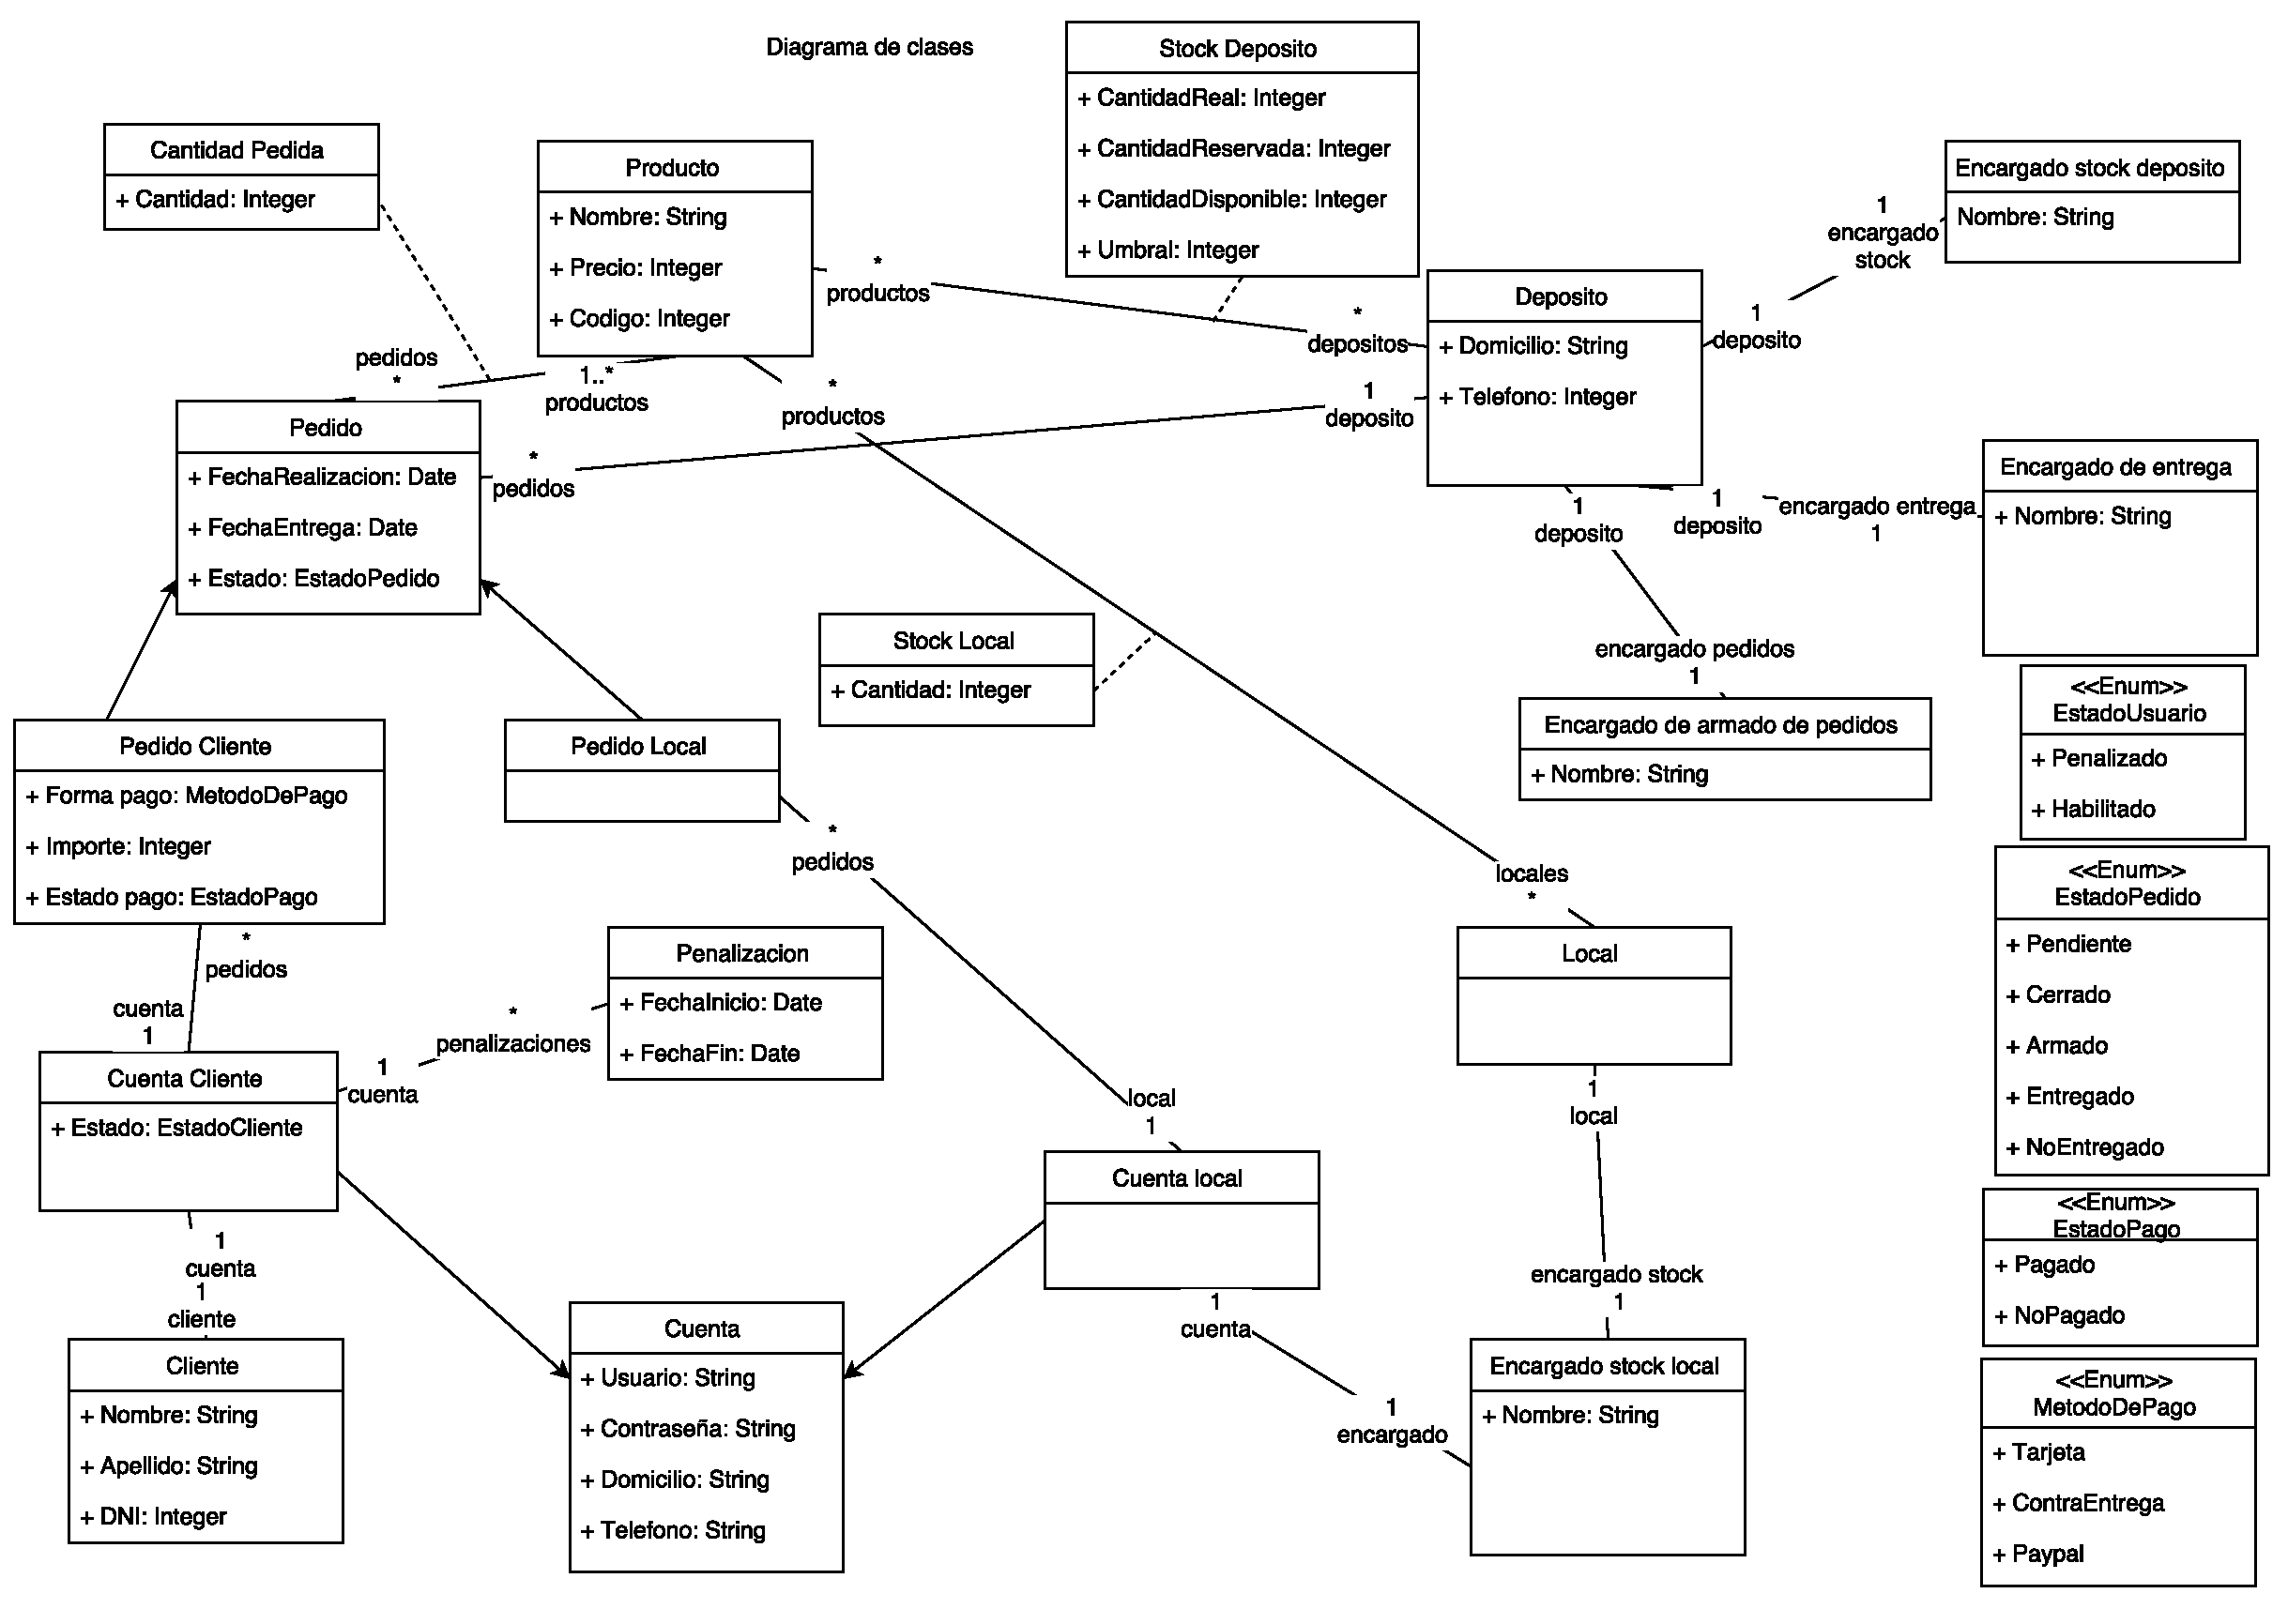
\includegraphics[scale=0.5, angle=90]{secciones/diagramaClases}
\newpage

\subsubsection{Restricciones OCL}

\begin{enumerate}
    \item Los clientes solo pueden tener un pedido activo a la vez.

    \begin{center}
    \begin{tabular}{p{0.2\textwidth} p{0.8\textwidth}}
        \textsc{Contexto} & Cuenta Cliente \\
        \textsc{Invariante} & \texttt{self.pedidos->select(p | p.Estado =
        Pendiente or p.Estado = Cerrado or p.Estado = Armado)->size() <= 1} \\
    \end{tabular}
    \end{center}

    \item Los locales solo pueden tener un pedido de reposición de stock activo a la vez.

    \begin{center}
    \begin{tabular}{p{0.2\textwidth} p{0.8\textwidth}}
        \textsc{Contexto} & Cuenta local \\
        \textsc{Invariante} & \texttt{self.pedidos->select(p | p.Estado =
        Pendiente or p.Estado = Cerrado or p.Estado = Armado)->size() <= 1} \\
    \end{tabular}
    \end{center}

    \item Calculo de la cantidad disponible de un producto en el stock de un deposito.

    \begin{center}
    \begin{tabular}{p{0.2\textwidth} p{0.8\textwidth}}
        \textsc{Contexto} & Stock Depósito \\
        \textsc{Invariante} & \texttt{self.CantidadDisponible = self.CantidadReal - self.CantidadReservada} \\
    \end{tabular}
    \end{center}

    \item La cantidad reservada de un producto en un deposito es igual a la suma de la cantidad pedida de ese producto en los pedidos activos realizados a dicho deposito.

    \begin{center}
    \begin{tabular}{p{0.2\textwidth} p{0.8\textwidth}}
        \textsc{Contexto} & Depósito \\
        \textsc{Invariante} & \texttt{self.Stock Deposito->forAll(sd | sd.CantidadReservada = self.pedidos->select(pe | pe.productos->exists(sd.Producto) and (pe.Estado = Pendiente or pe.Estado = Cerrado or pe.Estado = Armado))->collect((pe, sd.Producto).Cantidad)->sum()} \\
    \end{tabular}
    \end{center}
    
        \item La fecha de inicio de una penalización es anterior a su fecha de finalización.

    \begin{center}
    \begin{tabular}{p{0.2\textwidth} p{0.8\textwidth}}
        \textsc{Contexto} & Penalización \\
        \textsc{Invariante} & \texttt{self.FechaInicio <\ self.FechaFin} \\
    \end{tabular}
    \end{center}

    \item No puede haber pedidos por parte de un cliente con fecha dentro del
    rango de alguna penalización de esa cuenta.

    \begin{center}
    \begin{tabular}{p{0.2\textwidth} p{0.8\textwidth}}
        \textsc{Contexto} & Cuenta cliente \\
        \textsc{Invariante} & \texttt{self.pedidos->forAll(p |
        self.penalizaciones->forAll(pen | p.Fecha < pen.FechaInicio or p.Fecha > pen.FechaFin)} \\
    \end{tabular}
    \end{center}

    \item Los períodos de las penalizaciones de un cliente no pueden solaparse.

    \begin{center}
    \begin{tabular}{p{0.2\textwidth} p{0.8\textwidth}}
        \textsc{Contexto} & Cuenta cliente \\
        \textsc{Invariante} & \texttt{self.penalizaciones->forAll(p1, p2 |
        p1.FechaFin < p2.FechaInicio or p1.FechaInicio > p2.FechaFin)} \\
    \end{tabular}
    \end{center}

    \item Los productos de los pedidos atendidos por un depósito tiene que
    estar en el catálogo de dicho depósito.

    \begin{center}
    \begin{tabular}{p{0.2\textwidth} p{0.8\textwidth}}
        \textsc{Contexto} & Pedido \\
        \textsc{Invariante} &
        \texttt{self.deposito.productos->includesAll(self.productos)} \\
    \end{tabular}
    \end{center}


    \item Los pedidos de los locales no pueden estar marcados como no
    entregados.

    \begin{center}
    \begin{tabular}{p{0.2\textwidth} p{0.8\textwidth}}
        \textsc{Contexto} & Pedido local \\
        \textsc{Invariante} & \texttt{self.Estado <>\ NoEntregado} \\
    \end{tabular}
    \end{center}
    
    \item Definición de cuando un cliente esta penalizado.

    \begin{center}
    \begin{tabular}{p{0.2\textwidth} p{0.8\textwidth}}
        \textsc{Contexto} & Cuenta cliente \\
        \textsc{Invariante} & \texttt{if (self.penalizaciones->exists(p | p.FechaInicio <= now() <= p.FechaFin) then self.Estado = Penalizado else self.Estado = Habilitado endif)} \\
    \end{tabular}
    \end{center}
    
    \item Calculo del importe de un pedido.

    \begin{center}
    \begin{tabular}{p{0.2\textwidth} p{0.8\textwidth}}
        \textsc{Contexto} & Pedido Cliente \\
        \textsc{Invariante} & \texttt{self.Importe = self.Cantidad\ Pedida->collect(cp | cp.Cantidad * cp.Producto.Precio)->sum()} \\
    \end{tabular}
    \end{center}
    
     \item La fecha de entrega de un pedido debe ser igual o posterior a la fecha en la que se realizo el pedido.

    \begin{center}
    \begin{tabular}{p{0.2\textwidth} p{0.8\textwidth}}
        \textsc{Contexto} & Pedido \\
        \textsc{Invariante} & \texttt{self.FechaRealizacion <= self.FechaEntrega} \\
    \end{tabular}
    \end{center}
    
    \item Los pedidos entregados siempre son pagados.
    
    \begin{center}
    \begin{tabular}{p{0.2\textwidth} p{0.8\textwidth}}
        \textsc{Contexto} & Pedido Cliente \\
        \textsc{Invariante} & \texttt{self.Estado == ``Entregado'' implies self.Estado pago == ``Pagado''} \\
    \end{tabular}
    \end{center}
    
    \item Los pedidos que se pagan online con tarjeta o por Paypal siempre se marcan como pagados.
    
    \begin{center}
    \begin{tabular}{p{0.2\textwidth} p{0.8\textwidth}}
        \textsc{Contexto} & Pedido Cliente \\
        \textsc{Invariante} & \texttt{(self.Forma pago == ``Tarjeta'' or self.Forma pago == ``Paypal'') implies self.Estado pago == ``Pagado''} \\
    \end{tabular}
    \end{center}
    
    \item El stock reservado no puede superar al stock real del deposito.
    
    \begin{center}
    \begin{tabular}{p{0.2\textwidth} p{0.8\textwidth}}
        \textsc{Contexto} & Stock Deposito \\
        \textsc{Invariante} & \texttt{self.CantidadReservada <= self.CantidadReal} \\
    \end{tabular}
    \end{center}
    
    \item Los pedidos se entregan, a lo sumo, siete días después de haber sido realizados.
    
    \begin{center}
    \begin{tabular}{p{0.2\textwidth} p{0.8\textwidth}}
        \textsc{Contexto} & Pedido \\
        \textsc{Invariante} & \texttt{self.FechaEntrega - self.FechaRealizacion <= 7} \\
    \end{tabular}
    \end{center}

\end{enumerate}

\subsubsection{Generación de los reportes de ventas}

Para mostrar como se podría generar un reporte de ventas en este modelo conceptual presentamos tres ejemplos:

\begin{itemize}
\item \textbf{Productos mas vendidos}: Primero, tomamos los objetos de la clase ``Cantidad Pedida'' y, para cada producto, sumamos el valor del campo ``Cantidad'' de los objetos de la clase ``Cantidad Pedida'' que estén relacionados con el objeto de la clase ``Producto'' que representa al producto en cuestión. Luego, ordenamos esta lista de forma decreciente.
\item \textbf{Depósitos con mas pedidos}: Dado un deposito podemos obtener todos los pedidos realizados a este mediante su relación con la clase ``Pedido''. Luego, haciendo \textit{size()} al conjunto obtenido por esta relación podemos obtener la cantidad de pedidos de cada deposito. Así podemos armar un lista, con la cantidad de pedidos de cada deposito y, luego, ordenarla de forma decreciente.
\item \textbf{Métodos de pago}: Dado todo el conjunto de instancias de ``Pedido Cliente'', filtramos por cada método de pago ofrecido a los pedidos cuyo campo ``Forma de pago'' se corresponda con el método de pago deseado y, luego, contamos cuantas instancias tenemos para cada uno de los métodos.
\end{itemize}

\subsubsection{Trazabilidad}
A continuación listamos los requerimientos que se modelan con este diagrama.

\begin{itemize}
\item \textbf{Agregar depósitos al sistema:} se agrega una nueva  Clase Deposito 
\item \textbf{Cerrar un pedido desde la pagina web:} el objeto pedido cambia su estado a cerrado
\item \textbf{Tomar productos del pedido => Notificar pedido armado:}  El estado del pedido cambia a armado
\item \textbf{Configurar umbrales por producto en el sistema:}  stockDeposito.umbral = umbral configurado
\item \textbf{Incrementar stock cuando recibo reposición del proveedor:}  stockDeposito.cantidadReal se le incrementa el stock que se pidió
\item \textbf{Coordinar fecha de entrega:}  Pedido.fechaDeEntrega $=$ fecha que el cliente acuerda
\item \textbf{Se puede consultar los registros de las ventas:}  \textbf{informe}
\item \textbf{Se puede configurar los parámetros del reporte:}  \textbf{informe}
\item \textbf{Mantener listado de productos comprados:}  Pedido.productos si Pedido.estado = Pagado
\item \textbf{Mantener información de los medios de pagos utilizados:}  
\item \textbf{Los locales puedan registrarse:}  PedidoCliente.metodoDePago
\item \textbf{Los locales pueden modificar los pedidos no cerrados:}  si Pedido.estado != Cerrado entonces se modifican las relaciones con productos
\item \textbf{Los clientes pueden modificar los pedido no cerrados:}  si Pedido.estado != Cerrado entonces se modifican las relaciones con productos
\item \textbf{Un cliente pueda registrarse:}  se crea un nuevo objeto CuentaCliente
\item \textbf{Un cliente pueda seleccionar la fecha de entrega:}  Pedido.fechaDeEntrega = fecha que el cliente acuerda
\item \textbf{Un cliente pueda ingresar sus datos de contacto:}  atributos de clase Cuenta
\item \textbf{Reservar stock:}  StockDeposito.cantidadReservada igual al stock reservado
\item \textbf{Consultar pedidos armados:}  se muestran los pedidos tal que Pedido.estadoPedido = Armado
\item \textbf{Seleccionar pedido entregado:}   se modifica Pedido.estadoPedido = Entregado
\item \textbf{El cliente pago en contra-entrega => se notifica pago a contra-entrega:}    se modifica Pedido.estadoPedido = Pagado
\item \textbf{El cliente pago desde la pagina => se notifica el pago online:}  se modifica Pedido.estadoPedido = Pagado
\item \textbf{Llevar el conteo en base a los pedidos realizados de cuantos productos quedan:}  StockDeposito.cantidadDisponible
\item \textbf{Mantener historial de pedidos entregados y no entregados de un cliente:}  Instancias de la clase Pedido asociadas con una instancia de la clase Cuenta
\item \textbf{Rechazar pedido durante un tiempo:}  clase Penalizacion
\item \textbf{Pedido llega a la casa del cliente:}  PedidoCliente.estadoPedido = Entregado
\item \textbf{Cliente pague el pedido:}  PedidoCliente.estadoPedido = Pagado
\item \textbf{Ofrecer pago con PayPal:}  PedidoCliente.metodoDePago = PayPal
\item \textbf{Ofrecer pago con credito:}  PedidoCliente.metodoDePago = Tarjeta
\item \textbf{Ofrecer pago con debito:}  PedidoCliente.metodoDePago = Tarjeta
\item \textbf{Ofrecer pago con efectivo:}  PedidoCliente.metodoDePago = ContraEntrega
 
\end{itemize}

\newpage

\subsection{Finite State Machine - FSM}

\subsubsection{Diagramas de FSM}

Con los diagramas de máquinas de estado (Finite State Machine - FSM) decidimos modelar los comportamientos del sistema que \textbf{requerían sincronización}. Estos comportamientos se representan mediante eventos y estados, y flechas indicando que evento lleva a que estado. Estos eventos pueden realizarse bajo condiciones y modificar el valor de variables predefinidas. También se utilizaron variables de tipo timer que representan a cronómetros (el tiempo de cada timer transcurrirá en el estado que haga referencia a éste). 


Los comportamientos modelados son:
\begin{itemize}
\item El procesamiento de los pedidos de los clientes (creación, modificación, restricciones en las cantidades pedidas, etc).
\item La reserva del stock del depósito en respuesta al pedido de un cliente.
\item El funcionamiento de las alarmas de cada producto en cada depósito.
\item La penalización de los usuarios cuando no reciben un pedido.
\item La actualización del stock luego de un pedido al proveedor.
\end{itemize}


Tres cosas importantes que se deben ver en este modelo son:
\begin{itemize}
\item Cuando un cliente confirma su pedido (mediante ``Realiza un pedido''), el sistema reserva en el depósito el stock necesario para satisfacer dicho pedido y, en caso de no poder satisfacerlo, dicho pedido no es aceptado.
\item Al igual que en el caso de uso ``Modificando pedido'', no se permite que un cliente quite productos o unidades de un producto que ya pidió. Solo se le permite agregar productos o unidades. Esto es así porque los productos del pedido original pudieron ya haber sido cobrados al cliente.
\item Cuando un cliente está en su periodo de penalización, no es capaz de iniciar nuevos pedidos, es decir, el sistema los rechaza.
\end{itemize}

A continuación mostraremos las máquinas de estado realizadas, las cuales se sincronizan todas entre si para dar lugar al comportamiento completo del sistema:

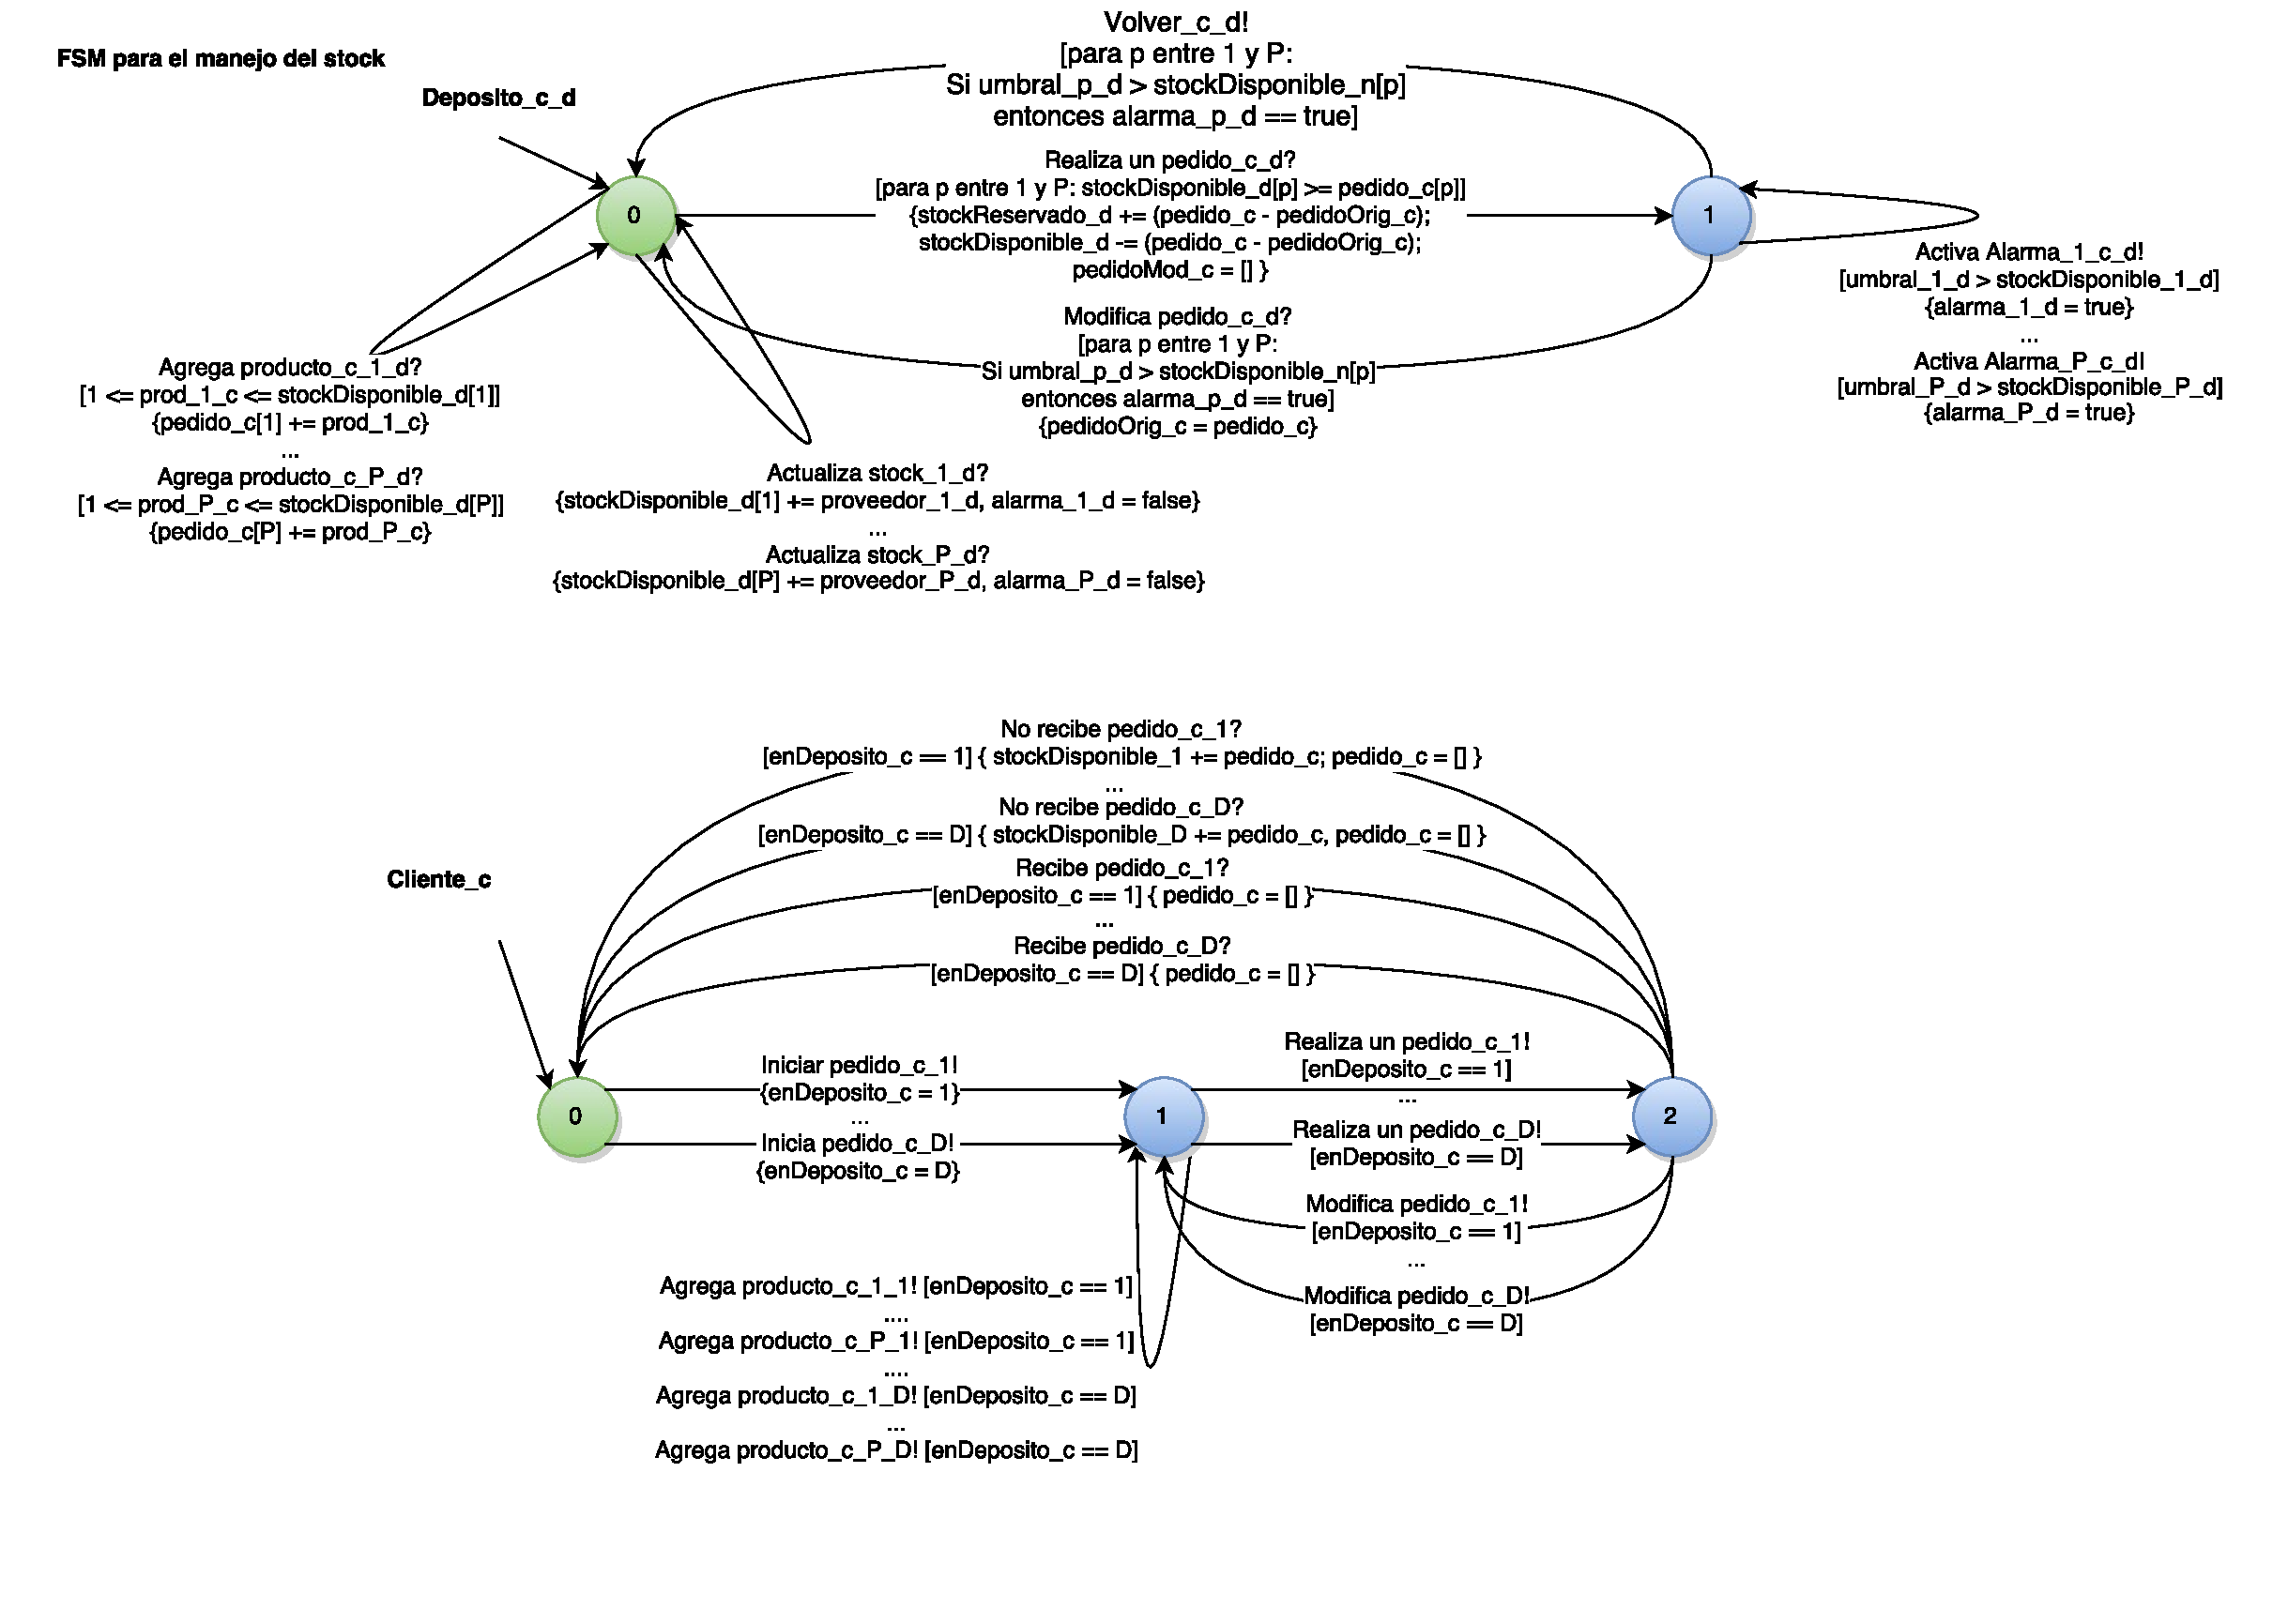
\includegraphics[scale=0.5, angle=90]{secciones/FSM}

\newpage

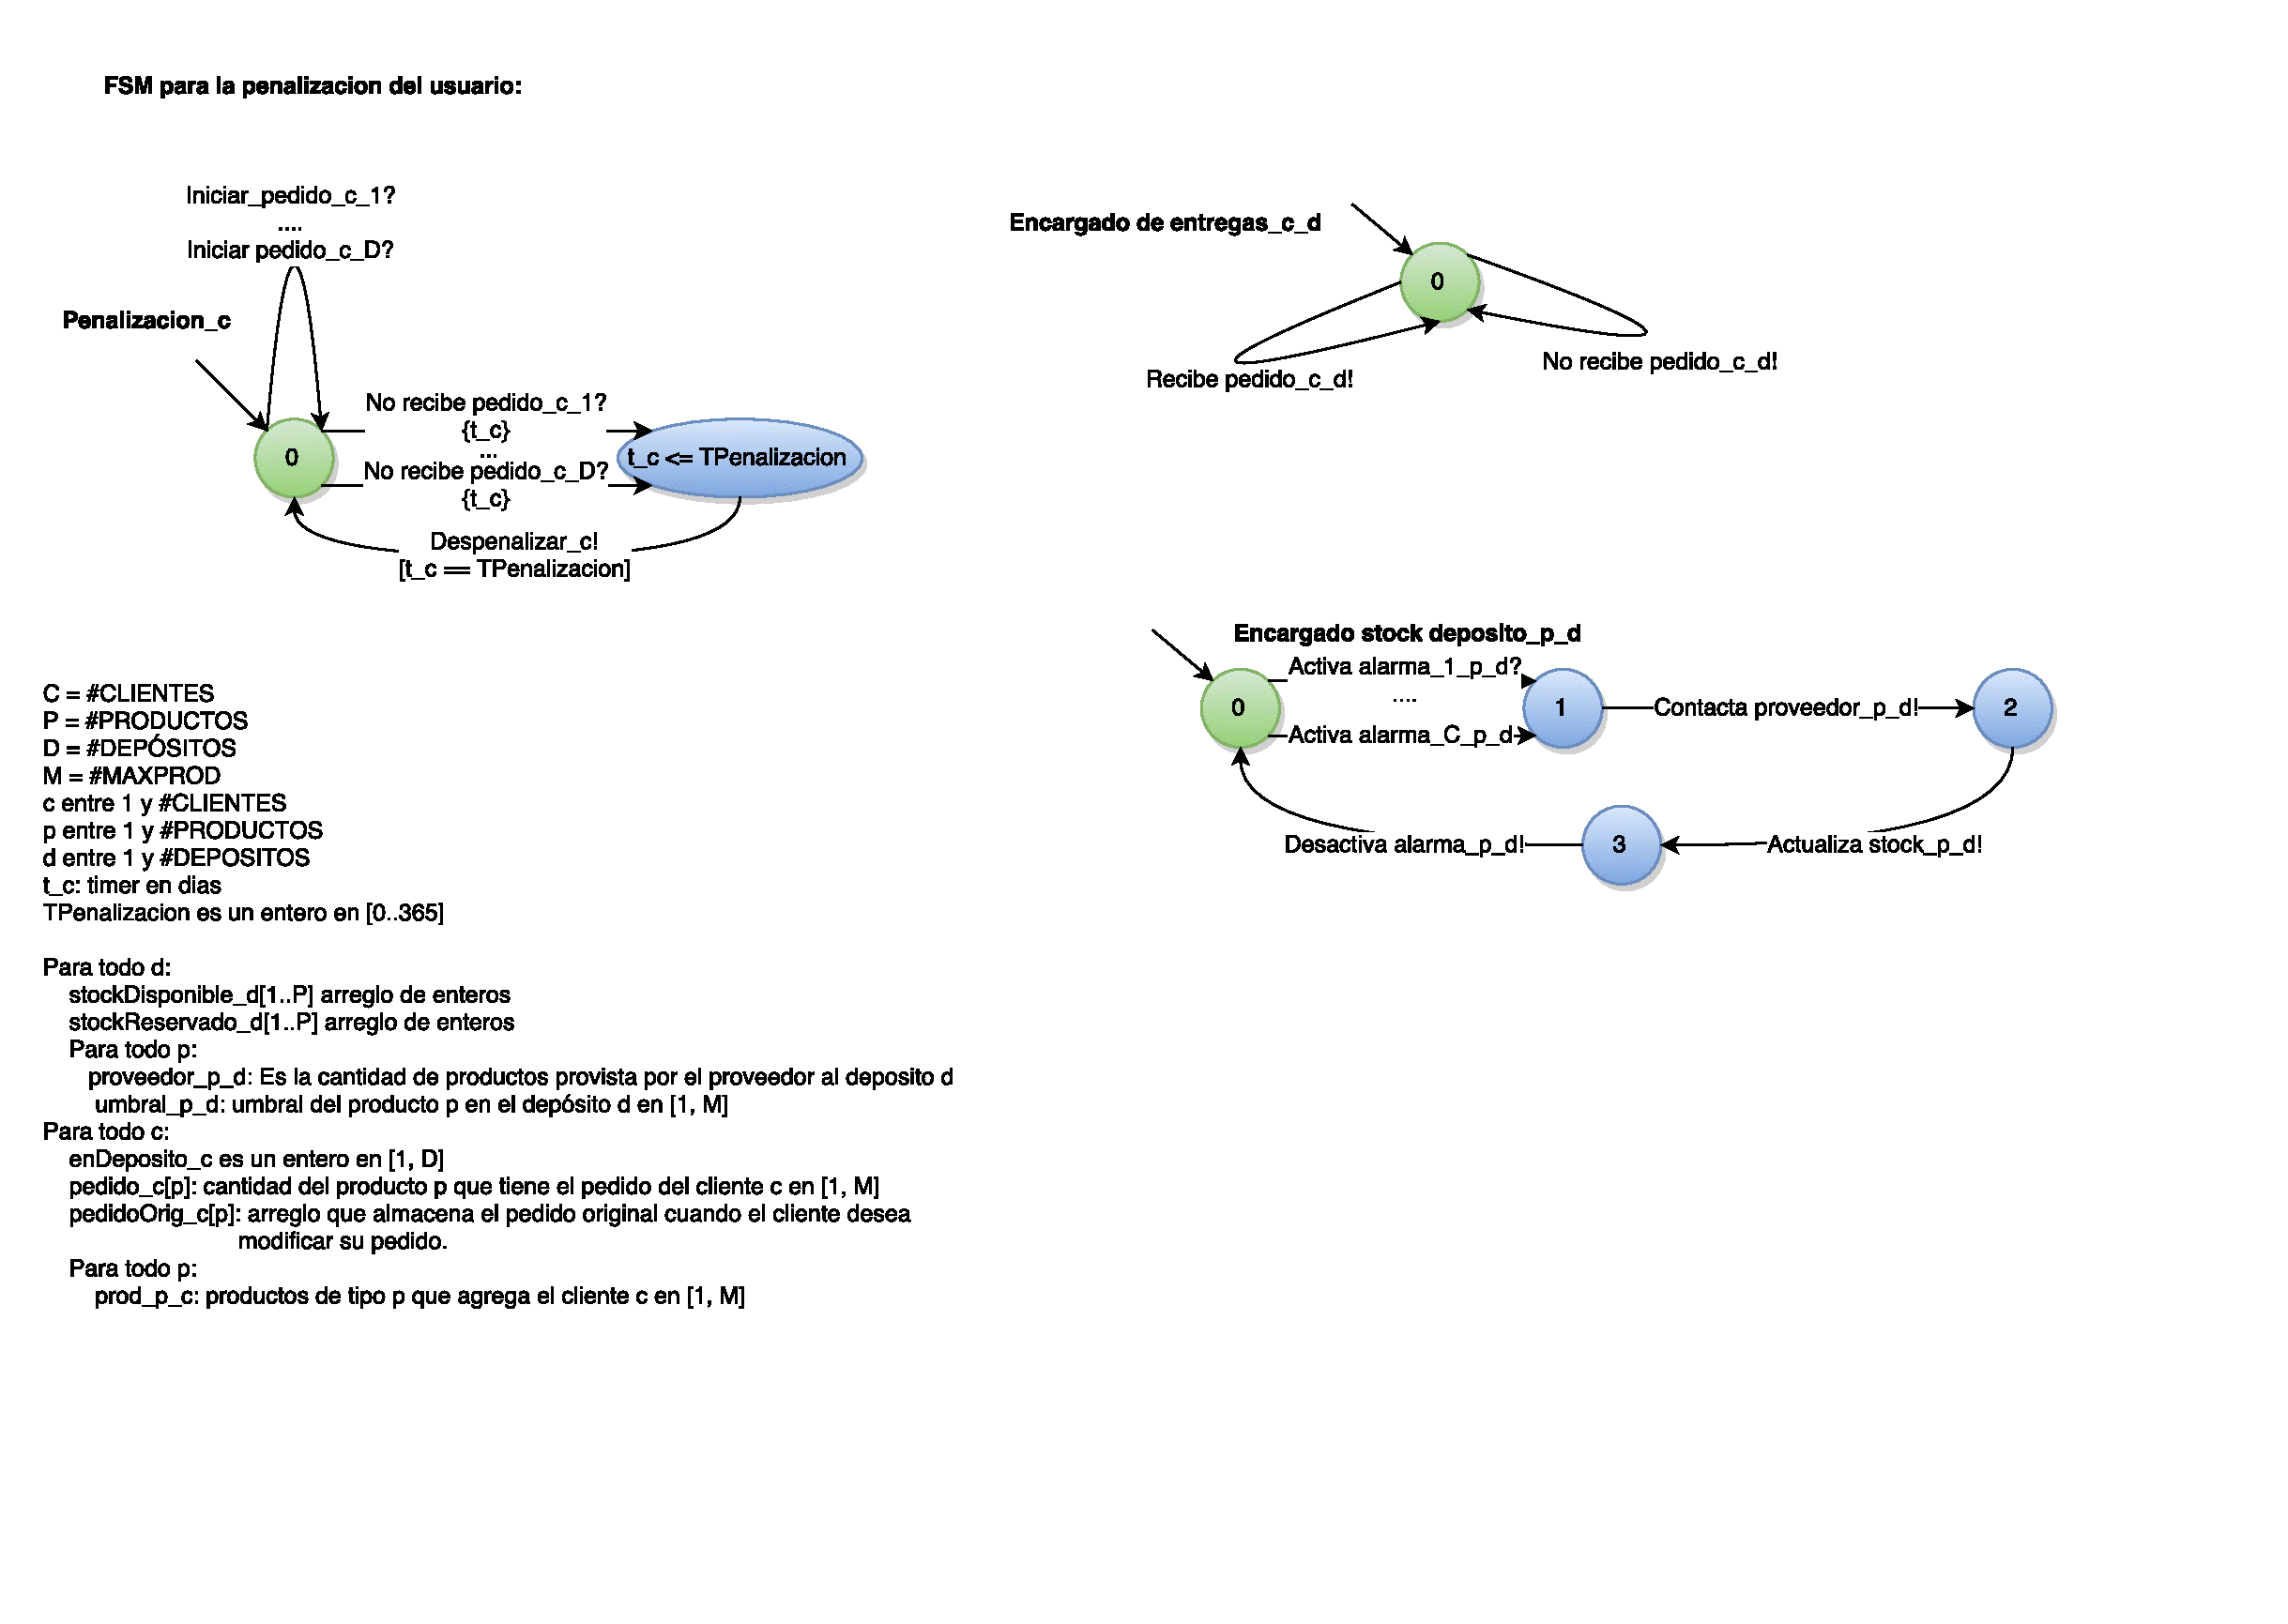
\includegraphics[scale=0.5, angle=90]{secciones/FSM2}

\newpage

El comportamiento del sitio web con respecto a un deposito esta dado por la composición paralela de:
\begin{center}
$Deposito_d$ = $Deposito\_1\_d$ || $Deposito\_2\_d$ || \ldots || $Deposito\_C\_d$.
\end{center}

El comportamiento del sistema de penalización de usuarios esta dado por la composición paralela de:
\begin{center}
$Penalizacion$ = $Penalizacion\_1$ || $Penalizacion_2$ || \ldots || $Penalizacion_C$
\end{center}

El comportamiento del encargado de entregas de un deposito esta dado por la composición paralela de:
\begin{center}
$Encargado\ de\ entregas\_d$ = $Encargado\ de\ entregas\_1\_d$ || $Encargado\ de\ entregas\_2\_d$ || \ldots || $Encargado\ de\ entregas\_C\_d$
\end{center}

El comportamiento del encargado de stock de un deposito esta dado por la composición paralela de:
\begin{center}
$Encargado\ de\ stock\ deposito\_d$ = $Encargado\ de\ stock\ deposito\_1\_d$ || $Encargado\ de\ stock\ deposito\_2\_d$ || \ldots || $Encargado\ de\ stock\ deposito\_P\_d$
\end{center}

El comportamiento completo del sistema esta dado por la composición paralela de:
\begin{center}
$Sistema$ = $Penalizacion$ || $Deposito\_1$ || \ldots || $Deposito\_D$ || $Encargado\ de\ entregas\_1$ || \ldots || $Encargado\ de\ entregas\_D$ || $Encargado\ de\ stock\ deposito\_1$ || \ldots || $Encargado\ de\ stock\ deposito\_D$ || $Cliente\_1$ || \ldots || $Cliente\_C$
\end{center}

\subsubsection{Trazabilidad}
A continuación listamos los requerimientos que se modelan con este diagrama:
\begin{itemize}
\item \textbf{Incrementar stock cuando recibo reposición del proveedor:} en la maquina encargado stock $deposito\_d$, la acción $actualizarStock\_d$
\item \textbf{Los clientes pueden y ver y seleccionar los productos que desean recibir:} maquina $Cliente\_c$, acción $agregaProducto\_c\_p\_d$
\item \textbf{Reservar stock:} maquina $Deposito\_d$, acción $realizaPedido\_c\_d$
\item \textbf{Los productos en falta son filtrado del listado que ve el cliente:} maquina $Deposito\_d$, acción $agregaProducto\_c\_p\_d$
\item \textbf{La cantidad máxima permitida para pedir un producto es igual a la que hay en el deposito:} maquina $Deposito\_d$, acción $agregaProducto\_c\_p\_d$
\item \textbf{Proveedor envía producto:} maquina $EncargadoStockDeposito\_d$, acción $actualizarStock\_d$
\item \textbf{Llevar el conteo en base a los pedidos realizados de cuantos productos quedan:}  array stockDisponible
\item \textbf{Se disparan alarmas cuando la cantidad de productos cae debajo del umbral configurado:} maquina $Deposito_d$, acción $activarAlarma\_p\_d$
\item \textbf{Contactar al proveedor:} $EncargadoStockDeposito\_d$, acción $contactarProveedor\_d$
\item \textbf{Rechazar pedido durante un tiempo:} $Penalizacion\_c$, segundo estado
\item \textbf{Pedido llega a la casa del cliente:} $EncargadoEntregas\_d$, acción $pedidoEnviado\_c\_d$
\end{itemize}

\newpage

\subsection{Modelo de comportamiento}

\subsubsection{Diagrama de actividad}

En este ultimo modelo mostraremos las actividades realizadas con su respectivo orden. Este orden lo indicaremos con flechas. También mostraremos los responsables de cada actividad. Las actividades también pueden suceder de forma concurrente. Para esto usaremos una barra (que llamaremos fork) y colocaremos las actividades concurrentes debajo de esta. Luego de esto hace falta que las actividades esperen a las que iniciaron el fork con ésta. Usaremos también una barra para esto, colocando las actividades por encima (que llamaremos join). Además se colocará condiciones if que indican a dónde se dirigirá un flujo que depende de esa condición.

Los flujos que se observan son:
\begin{itemize}
\item El flujo de un pedido de un cliente y de un local desde que es realizado hasta que es entregado o no a su domicilio.
\item El flujo de reponer el stock de un depósito desde que se arma el pedido para el proveedor hasta que este los envía y se actualiza el stock en consecuencia.
\end{itemize}

En estos tres flujos se puede observar el orden en el que son realizados muchos de los casos de uso que se mostraron en el primero modelo.

A continuación presentamos los tres diagramas de actividad realizados:

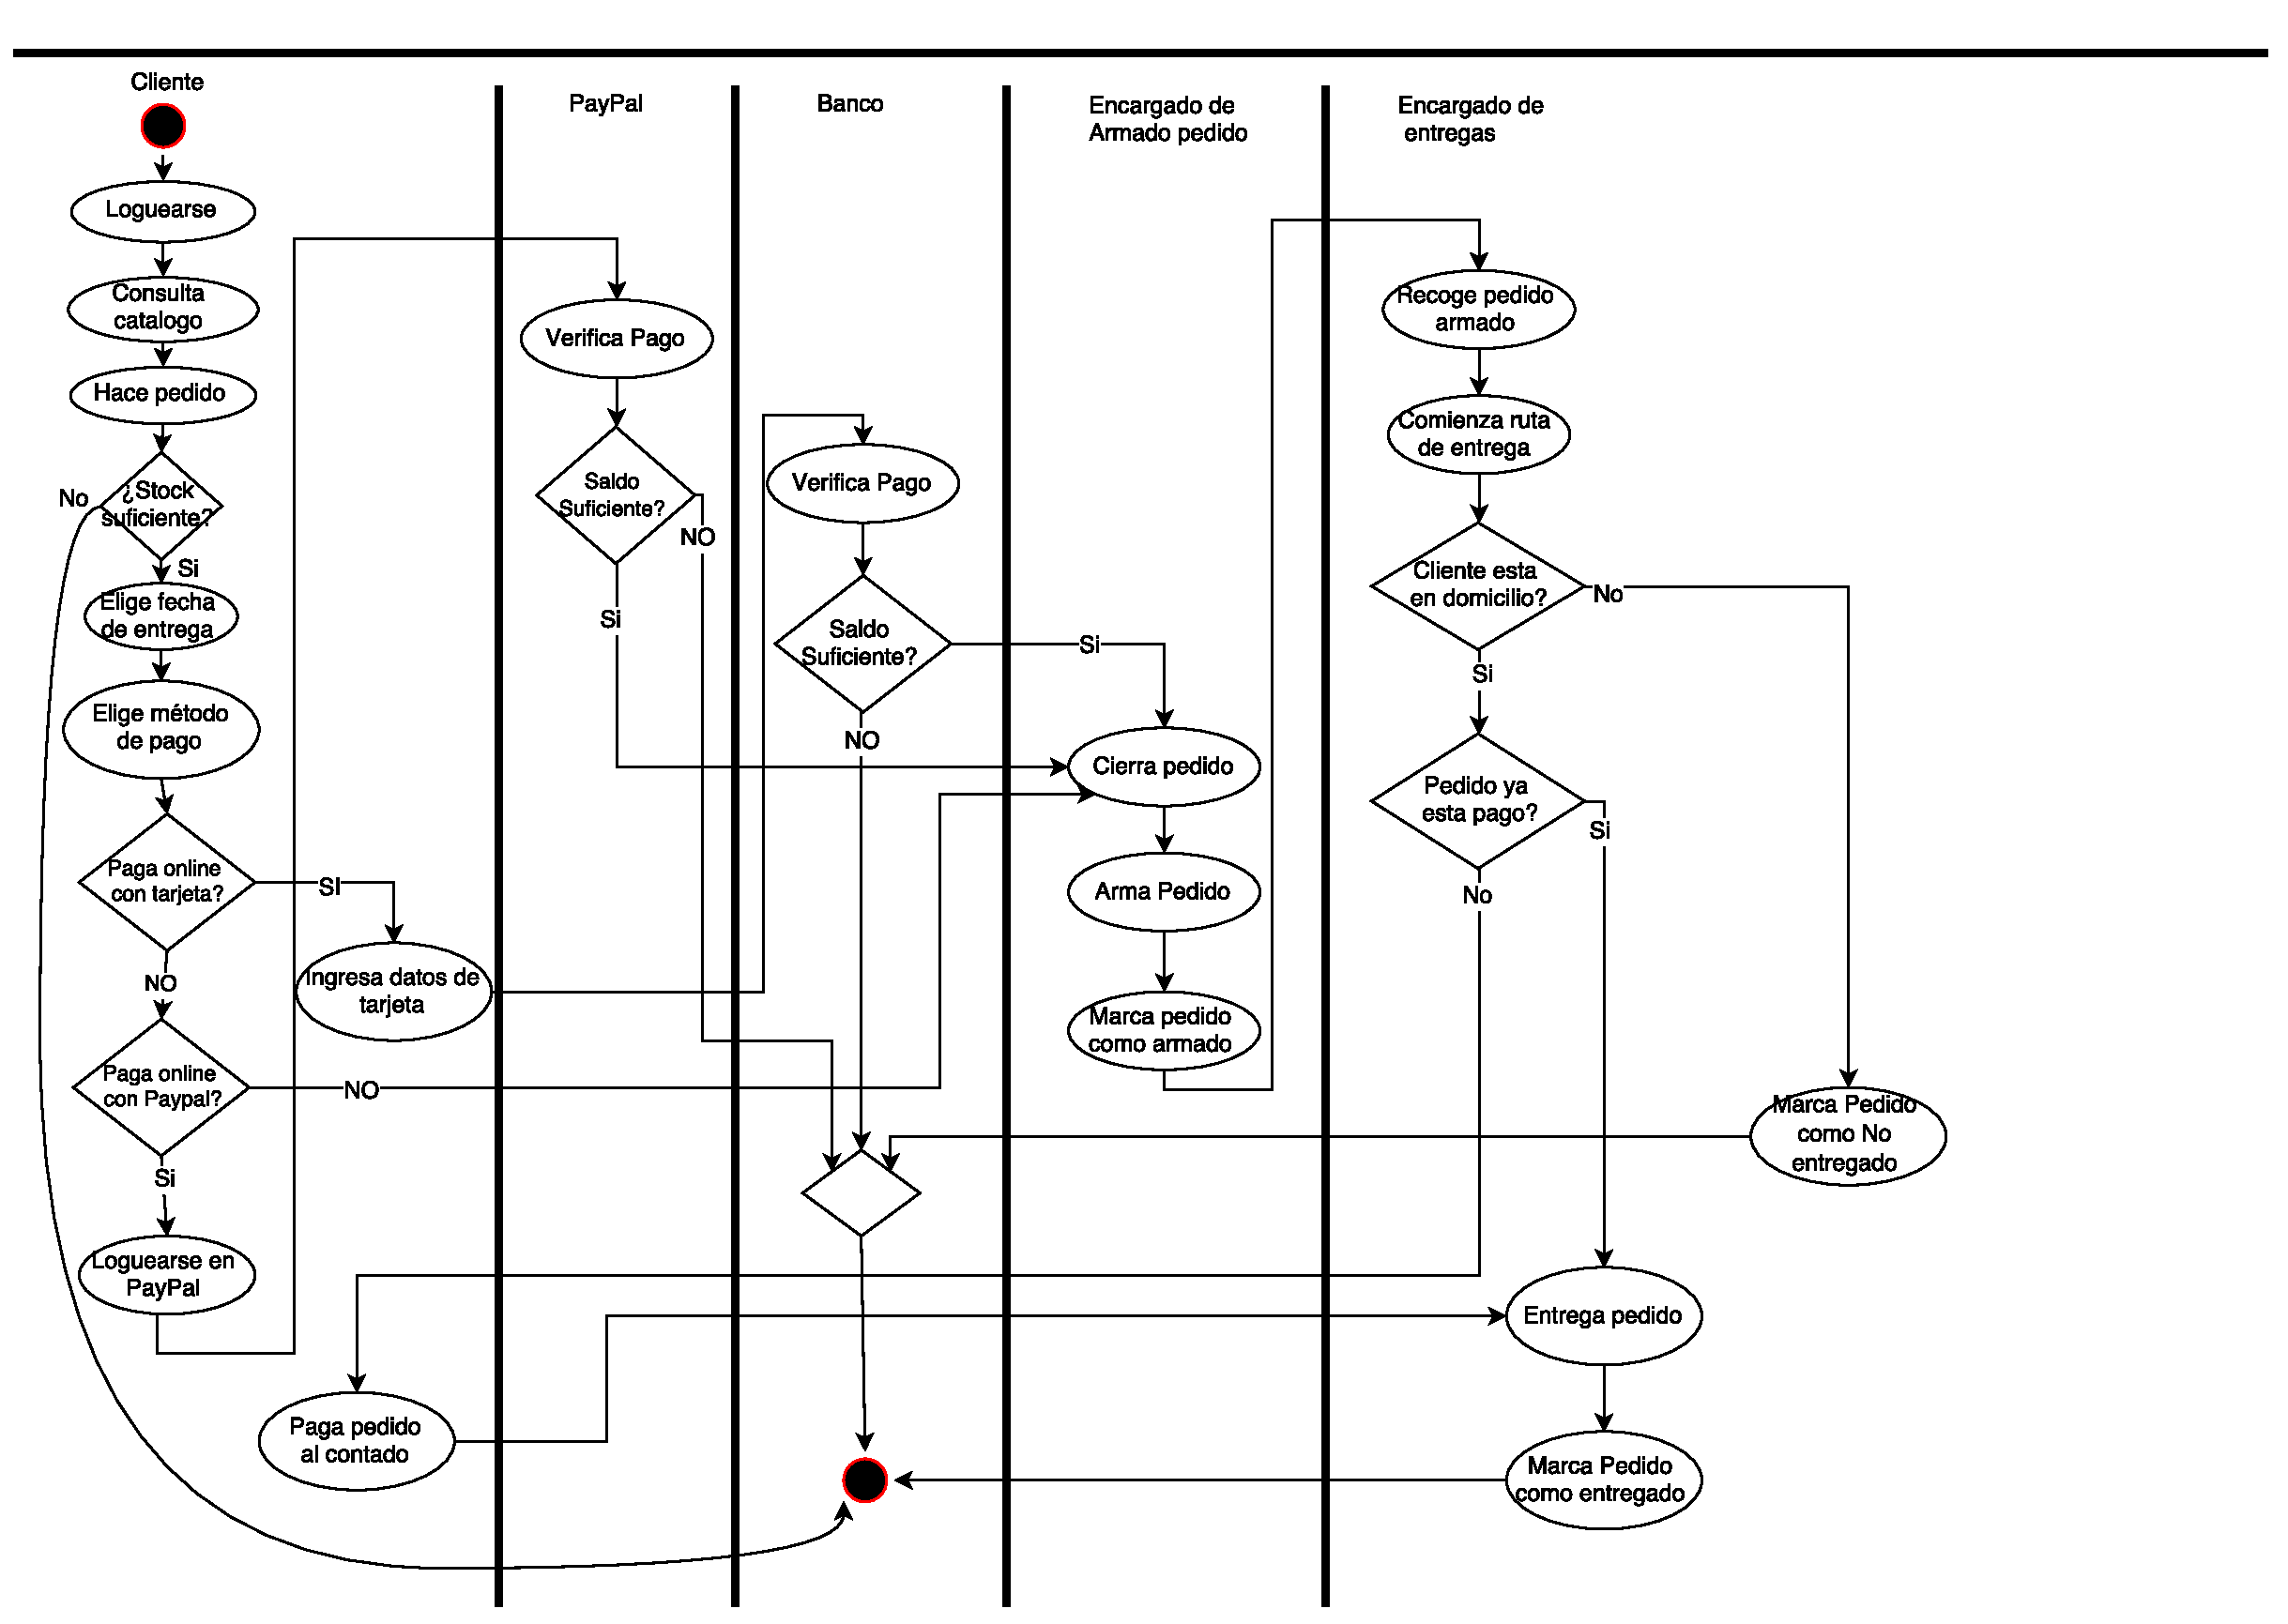
\includegraphics[scale=0.5, angle=90]{secciones/diagramaActividad1}
\newpage
\newpage
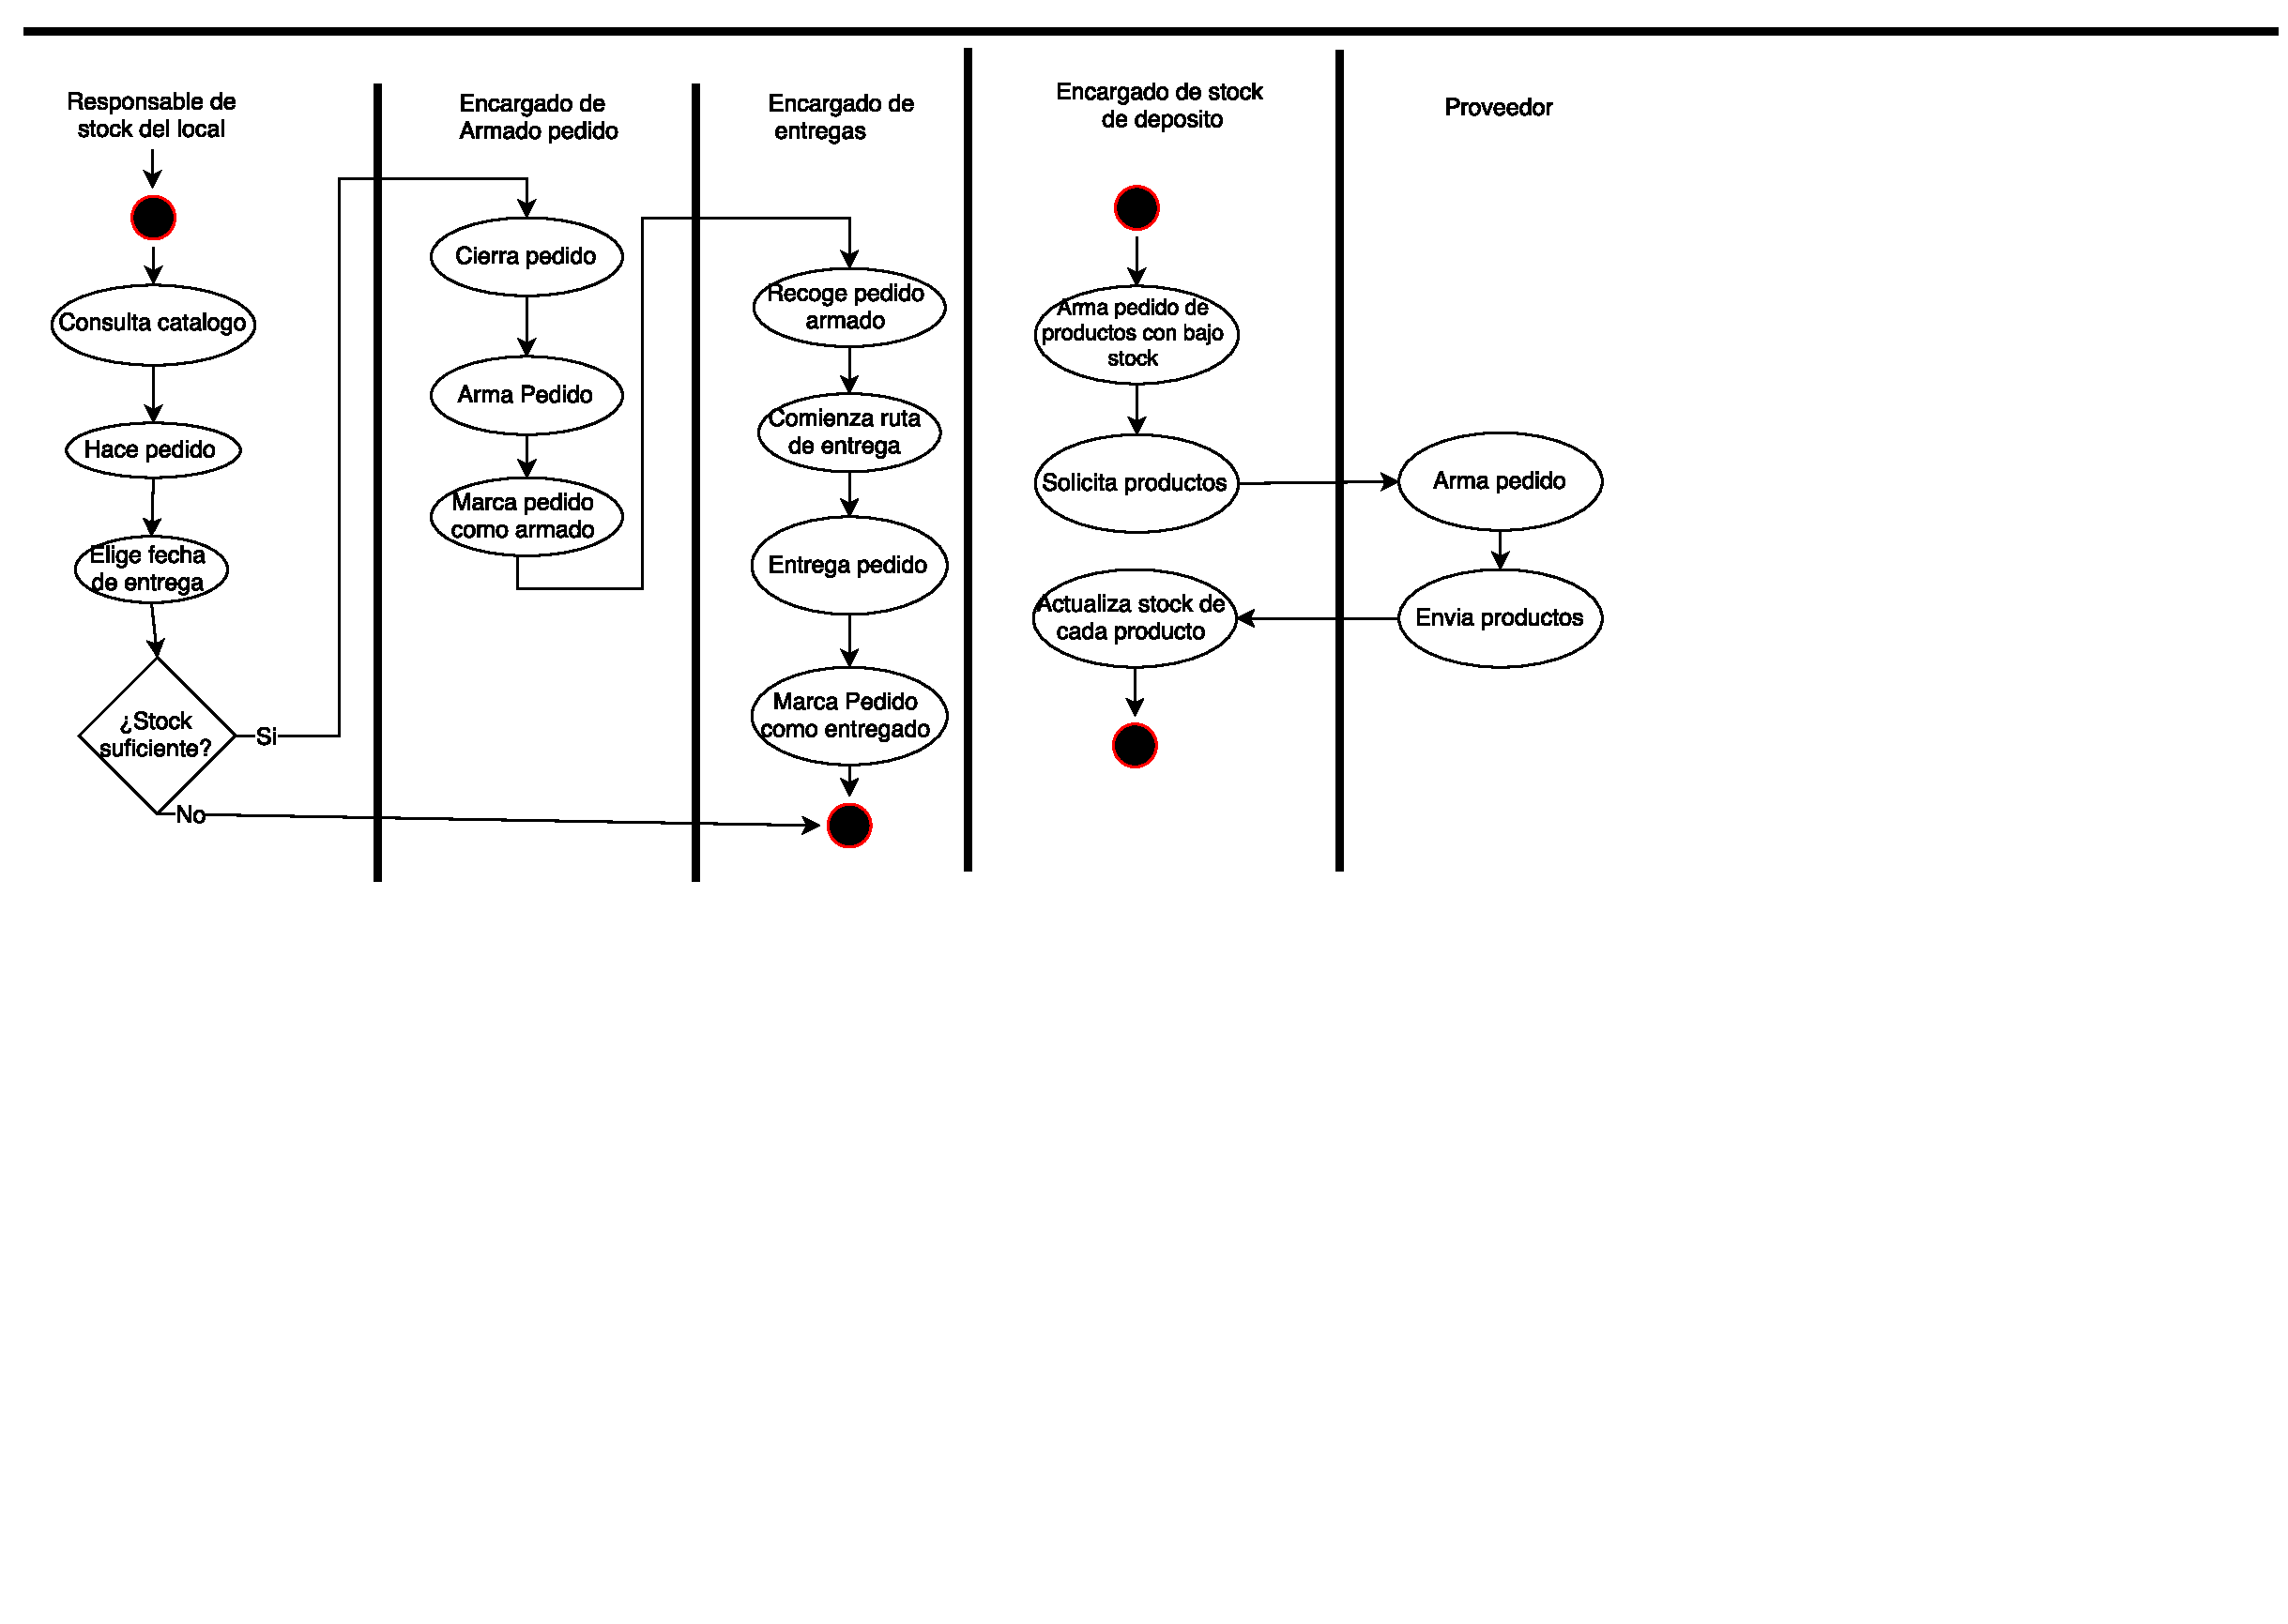
\includegraphics[scale=0.5, angle=90]{secciones/diagramaActividad2}

\newpage

\subsubsection{Trazabilidad}
A continuación listamos los requerimientos que se modelan con este diagrama.

\begin{itemize}
\item \textbf{Los usuarios se pueden autentificar:} Actividad loguearse
\item \textbf{Cerrar un pedido desde la pagina web:} Actividad Cierra pedido
\item \textbf{Tomar productos del pedido => Notificar pedido armado:} Actividad Marca pedido como armado
\item \textbf{Coordinar fecha de entrega:} Actividad Elije fecha
\item \textbf{Los locales pueden y ver y seleccionar los productos que desea recibir:} Actividad Consultar Catalogo
\item \textbf{Un cliente pueda seleccionar la fecha de entrega:} Actividad Elije fecha  de entrega
\item \textbf{Entregar pedidos al local:} Flujo de un pedido de un local
\item \textbf{Seleccionar pedido entregado:} Actividad Marca pedido como entregado
\item \textbf{El cliente pago en contra-entrega => se notifica pago a contra-entrega:} Actividad Paga pedido al contado
\item \textbf{El cliente pago desde la pagina => se notifica el pago online:} Actividad Loguearse en PayPal e Ingresando datos tarjeta
\item \textbf{Coordinar fecha de entrega con proveedor:} Actividad Solicita productos
\item \textbf{Ofrecer pago con PayPal:} Actividad Logueandose en PayPal
\item \textbf{Ofrecer pago con crédito:} Actividad Ingresando datos tarjeta
\item \textbf{Ofrecer pago con débito:} Actividad  Ingresando datos tarjeta
\item \textbf{Ofrecer pago con efectivo:} Actividad Paga pedido al contado

\end{itemize}

\newpage

\subsection{Trazabilidad}
Para mostrar la trazabilidad y la completitud de nuestros diagramas, armamos una tabla con los requerimientos y las presunciones del dominio aclarando para cada uno en que diagrama se ve reflejado. Luego en cada diagrama en particular se detalla cada requerimiento o presunción del dominio.
\begin{center}
\begin{table}[H]
\begin{tabular}{|l|l|l|}
\hline
\# & Requerimiento & Diagrama   \\ \hline
1  & Reponer los productos en las góndolas & \\ \hline
2  & Agregar depósitos al sistema & CU - MC \\ \hline
3  & Los usuarios se pueden autentificar. & CU - DA \\ \hline
4  & Que el cliente envié una copia del DNI mediante el sitio. & CU \\ \hline
5  & Cerrar un pedido desde la pagina web & CU - MC - DA \\ \hline
6  & Tomar productos del pedido => Notificar pedido armado. & CU - MC - DA \\ \hline
7  & Configurar umbrales por producto en el sistema. & CU - MC \\ \hline
8  & Incrementar stock cuando recibo reposición del proveedor. & CU - MC - FSM \\ \hline
9  & Coordinar fecha de entrega. & CU - MC - DA \\ \hline
10  & Se puede consultar los registros de las ventas.  & CU - MC \\ \hline
11  & Se puede configurar los parámetros del reporte. & CU - MC \\ \hline
12  & Mantener listado de productos comprados. &  MC \\ \hline
13  & Mantener información de los medios de pagos utilizados. & MC \\ \hline
14  & Los locales puedan registrarse. & CU - MC  \\ \hline
15  & Los locales pueden y ver y seleccionar los productos que desea recibir. & CU  - DA  \\ \hline
16  & Los locales pueden modificar los pedidos no cerrados. & CU - MC  \\ \hline
17  & Los clientes pueden y ver y seleccionar los productos que desean recibir. & CU  - FSM \\ \hline
18  & Los clientes pueden modificar los pedido no cerrados. & CU - MC  \\ \hline
19 & Un cliente pueda registrarse. & CU - MC  \\ \hline
20  & Un cliente pueda seleccionar la fecha de entrega. & CU - MC - DA  \\ \hline
21  & Un cliente pueda ingresar sus datos de contacto. & CU - MC  \\ \hline
22  & Reservar stock. & CU - MC - FSM \\ \hline
23  & Los productos en falta son filtrado del listado que ve el cliente. & CU  - FSM \\ \hline
24  & {\scriptsize La cantidad máxima permitida para pedir un producto es igual a la que hay en el deposito}. & CU  - FSM \\ \hline
25  &  {\scriptsize Lograr que la interfase funcione correctamente en computadoras de escritorio} &  \\ \hline
26  & Lograr que la interfase funcione correctamente en dispositivos móviles &  \\ \hline
27  & Entregar pedidos al local & DA \\ \hline
28  & Consultar pedidos armados & CU - MC  \\ \hline
29  & Seleccionar pedido entregado & CU - MC - DA  \\ \hline
30  & El cliente pago en contraentrega => se notifica pago a contraentrega. & CU - MC - DA  \\ \hline
31  & El cliente pago desde la pagina => se notifica el pago online. & CU - MC - DA \\ \hline
32  & Coordinar fecha de entrega con proveedor. & CU - DA  \\ \hline
33  & Proveedor envía producto & FSM \\ \hline
34  &  {\scriptsize Llevar el conteo en base a los pedidos realizados de cuantos productos quedan.} & CU - MC  - FSM \\ \hline
35  &  {\scriptsize Se disparan alarmas cuando la cantidad de productos cae debajo del umbral configurado}  & FSM \\ \hline
36 & Contactar al proveedor. & FSM \\ \hline
\end{tabular}
\end{table}
\end{center}


\begin{center}
\begin{table}[H]
\begin{tabular}{|l|l|l|}
37  &  {\scriptsize Poder definir si un cliente es malo en función de un porcentaje de pedidos no entregados.} &  \\ \hline
38  & Mantener historial de pedidos entregados y no entregados de un cliente.  & MC \\ \hline
39  & Incrementar el precio del próximo pedido. &  \\ \hline
40  & Rechazar pedido durante un tiempo & MC - FSM \\ \hline
41  & Pedido llega a la casa del cliente & MC - FSM \\ \hline
42  & Cliente pague el pedido & CU - MC  \\ \hline
43  & Ofrecer pago con PayPal & CU - MC - DA \\ \hline
44  & Ofrecer pago con crédito & CU - MC - DA \\ \hline
45  & Ofrecer pago con débito & CU - MC - DA  \\ \hline
46  & Ofrecer pago con efectivo.  & CU - MC - DA  \\ \hline
\end{tabular}
\end{table}
\end{center}

\textit{CU}: Diagrama de casos de uso.

\textit{MC}: Diagrama de clases - Modelo conceptual.

\textit{FSM}: Maquina de estados.

\textit{DA}: Diagrama de actividad.

\newpage

% - Vistas: está sería la parte principal del TP. Acá irían los diagramas y los escenarios representativos de uso. No necesariamente tiene que ser una gran sección, sino que pueden partirla por funcionalidades y a su vez por tipo de vista o de la forma que crean más pertinente. Esta sección NO DEBE SER una simple seguidilla de figuras sueltas. Debe estar acompañada de tantas explicaciones como sean necesarias para que se aprecie un hilo conductor.


\section{Discusión}

\subsection{Modificación de los pedidos}

Decidimos que tanto clientes como locales no puedan quitar productos de su pedido originales al momento de modificarlos.

En el caso de los pedidos de los clientes, lo que motivo esta decisión fue el hecho de que, si el cliente selecciono pagar su pedido original de forma online con tarjeta o Paypal, entonces todos los productos de dicho pedido ya fueron comprados. Entonces, si permitiéramos que el cliente quite productos de su pedido, podría darse el caso en que el cliente modificara su pedido de forma tal que el nuevo pedido tenga un importe menor que el abonado originalmente. En dicho caso tendríamos dos formas posibles de actuar:

\begin{itemize}
	\item Reembolsar al cliente la diferencia.
	\item Quedarnos con la diferencia de dinero.
\end{itemize}

La primer opción nos parece un tanto ilógica e incomoda desde un punto de vista comercial y la segunda opción nos parece deshonesta.

A pesar de contar con estas dos opciones, nosotros consideramos que el hecho de que el cliente realice un pedido establece un \textbf{contrato o compromiso} entre las dos partes \textit{(el cliente y Mes\%)}, en el cual el cliente se compromete a pagar los productos y la cadena Mes\% garantiza tener en stock los productos pedidos y entregarlos en tiempo y forma. Por ende, no permitimos que los clientes quiten productos de sus pedidos.

Agregar productos al pedido no implica ninguna modificación al \textit{contrato} previo, solo es un nuevo contrato al cual Mes\% se compromete a entregar en la misma fecha que el anterior.

Por otra parte, tampoco permitimos que los locales quiten productos de su pedido y esto es debido a como funciona el sistema de alarmas \textit{(avisos por mail)} de falta de stock de los producto. \textbf{Este mismo motivo también aplica a los pedidos de los clientes}.

Supongamos el siguiente escenario: Un pedido de un local causa que el stock de el producto X caiga por debajo del umbral configurado. Esto causara que se active la alarma asociada a dicho producto y que se envíe un mail al encargado de stock del deposito. Al recibir la notificación el encargado de stock realiza un pedido al proveedor para reponer las unidades del producto en falta. Supongamos ahora que el local es capaz de quitar productos de su pedido y decide quitar \textbf{todas} las unidades que solicito del producto X, causando así que el stock disponible en el deposito supere al umbral. Ahora, tenemos dos escenarios posibles:
\begin{itemize}
	\item Los nuevos pedidos que arriban al sistema causan que el stock del producto X vuelva a caer por debajo del umbral, enviándose un nuevo aviso al encargado de stock del deposito. Esto causaría que el sistema de alarmas se vuelva confuso para el encargado del stock, ya que podría darse el caso en que el stock del producto este cruzando de un lado al otro del umbral constantemente \textit{(por modificaciones en los pedidos)} y que el encargado reciba una cantidad absurda de notificaciones.
	\item No se reciben nuevos pedidos solicitando al producto X. Luego, arriba el pedido hecho al proveedor y ahora se tiene una cantidad muy grande de unidades del producto X que bien podrían: no venderse, producir problemas de espacio en el deposito, echarse a perder \textit{(si es que es algo perecedero)}, etc.
\end{itemize}

Ninguno de los dos escenarios nos parece tolerable, de modo que este motivo nos llevo a no permitir que los locales quiten productos de sus pedidos y es un motivo mas para que los clientes no puedan hacerlo.
 
\subsection{Rechazo de los pedidos}

Si el sistema no cuenta con el stock suficiente \textit{(definido como stock real menos stock reservado)} para satisfacer el pedido de un cliente en su totalidad, entonces se rechazara su pedido.

Esto se desprende directamente del enunciado, el cual nos indica que: ``No podemos tener problemas de stock cuando un pedido se realiza de forma online''.

Esto nos causa un pequeño inconveniente, el cual es: El usuario ve el stock disponible con el que cuenta el deposito al momento de \textbf{iniciar} su pedido, pero este valor puede diferir \textit{(haber disminuido)} al momento en que el usuario quiere confirmar su pedido, causando que el sistema se lo rechace y que el usuario haya perdido tiempo de su vida.

Creemos que este inconveniente no es muy grave y, si el deposito cuenta con cantidades de stock lo suficientemente grandes \textit{(y umbrales bien configurados)} como para que el pedido de un usuario no represente una diferencia para el resto de los usuarios comprando, entonces este escenario no sucederá frecuentemente.

\subsection{Pedidos no entregados}

Si al enviar un pedido a un cliente este no se encuentra en su domicilio, entonces se informa que el pedido no pudo ser entregado y los productos vuelven al deposito.
Ahora, existe la posibilidad de que el cliente haya pagado online el pedido antes de recibirlo, en cuyo caso tenemos tres formas de actuar:
\begin{itemize}
	\item Devolverle al cliente su dinero.
	\item Quedarnos con el dinero del cliente y con los productos del pedido.
	\item Quedarnos con el dinero del cliente y hacer que este vaya al deposito a buscar su pedido.
\end{itemize}

Nosotros optamos por la segunda opción, ya que es la mas conveniente para Mes\%. Pero, puede que esto no sea legal en algunos lugares, en cuyo caso creemos que se debería optar por la tercer opción, ya que es la que menos gastos y molestias le ocasionarían a Mes\%. En caso de elegir esta opción, seria necesario agregar una interacción entre el cliente y el encargado del deposito donde este le solicita su pedido y el encargado se lo entrega. Además de que se debería tener en mente el problema de espacio que esto podría ocasionar y de que forma el encargado de stock del deposito sabe que pedido corresponde a que cliente. También seria necesario agregar un caso de uso en donde, luego de entregarle el pedido al cliente, el encargado de stock del deposito lo marque como ``Pedido entregado''.

La primer opción queda descartada por lo ya dicho en la sección ``Modificación de los pedidos'', sobre que los pedidos son \textbf{contratos}. Además, desde un punto de vista comercial, seria realmente contraproducente devolver el dinero del pedido y además haber perdido dinero en el envió fallido del mismo.


\subsection{Fechas de entrega de los pedidos}

El sistema propone a los usuarios tres fechas al azar, en días hábiles, dentro de los siete días siguientes a la fecha en que se realizo el pedido.

Esto podría ocasionar que muchos pedidos se agenden para un mismo día pero, dado que la logística de la entrega de los pedidos no corre por nuestra cuenta y que no se nos impuso ninguna restricción sobre la cantidad de pedidos que se pueden entregar por día, asumimos que esto no ocasiona un problema y que los pedidos van a poder ser entregados.

En caso de que esto ocasionara un problema, podría resolverse fácilmente estableciendo un limite a la cantidad de pedidos \textit{(valor que desconocemos)} agendados por día y rechazando los pedidos de los usuarios si, a partir de la fecha actual, sucede que los próximos siete días alcanzaron su tope de pedidos para entregar.

% Debe contener un análisis general de las distintas alternativas y su impacto en los objetivos blandos. NO DEBE SER una lista de lo que ya se puede desprender del diagrama. Debe ser un análisis más cualitativo y "a vuelo de pájaro" que permita entender este asunto en pocas palabras. Esta sección también es ideal para que vuelquen las cosas que puedan haberles quedado "flojas" o no cerradas del todo: por ejemplo los potenciales conflictos entre objetivos, los aspectos que podrían hacer que todo el sistema no funcione como desean, etc.

\section{Conclusiones}

Este trabajo no resulto nada sencillo ya que implicaba realizar muchos diagramas, los cuales estaban estrechamente relacionados, y debían ser consistentes entre si y con lo realizado en el trabajo anterior.

Desde nuestro punto de vista, el diagrama de \textbf{casos de uso} debería haberse realizado en el primer trabajo conjuntamente con los diagramas de contexto, ya que estos tienen una muy fuerte relación y permiten detectar fácilmente errores o inconsistencias entre si. 

También creemos que el escribir los detalles de cada operación de los casos de uso ayuda enormemente a determinar el alcance del sistema, las cosas que necesitamos especificar, cómo se realizan y las cosas que podemos delegar a terceros, etc; y todo esto habría ayudado a la hora de diseñar el diagrama de objetivos, ya que mientras se escribe el detalle de una operación se piensa en diferentes formas de llevarla a cabo \textit{(posibles o-refinamientos)}.

El diagrama de clases nos ayudo mucho a comprender con que información iba a trabajar nuestro sistema, que información necesitábamos guardar y cual debíamos mantener actualizada.

Las máquinas de estado fueron un verdadero \sout{dolor de cabeza} reto, ya que realizar la sincronización de los pedidos de los usuarios de forma que todos puedan realizar pedidos sin importar el estado de los otros usuarios fue, como minino, muy complicado. A esto, además, se suma el hecho de que la maquina debía reflejar como el sistema mantenía actualizado el stock disponible y stock reservado del deposito en el que se hacia el pedido y el manejo de las alarmas una vez que el stock disponible caía por debajo de cierto umbral. Todo el proceso de desarrollar la FSM nos permitió notar algunas falencias en los detalles de algunos casos de uso \textit{(en el que el cliente realiza el pedido)}.

Los diagramas de actividad no aportaron mucho al entendimiento general del problema ni a detectar algún error. Además fueron los primeros diagramas en estar terminados y, por mucha diferencia, los que mas rápido se hicieron.

Finalmente, todo este proceso de muchas, muchas y muchas horas nos llevo a entender la dificultad de encarar un proyecto símil a un proyecto real \textit{(aunque claramente acotado)} y de la gran cantidad de decisiones que se deben tomar durante la etapa de diseño.

Creemos que seria sumamente útil contar con un software que se encargara de validar los diferentes diagramas \textit{(al menos hasta cierto punto)}, chequear inconsistencias entre estos y/o sugerir cambios.

Como nota final, creemos que el tener que atar nuestra solución al diagrama de objetivos realizado en el primer trabajo nos limito en este trabajo a la hora de tomar decisiones, ya que al momento de realizar el diagrama de objetivos hubo muchas situaciones \textit{(como el hecho de que no entregar un pedido ni devolver el dinero fuera ilegal o como asignar las fechas de entrega a los pedidos)} que no tuvimos en cuenta.

% Mencionar brevemente de qué formas les resultó más sencillo encarar el TP. Por ejemplo en qué orden realizaron los diagramas, qué aspectos presentaron las mayores dificultades, etc.

\end{document}

